%% LyX 2.4.3 created this file.  For more info, see https://www.lyx.org/.
%% Do not edit unless you really know what you are doing.
\documentclass[journal,article,submit,pdftex,moreauthors]{Definitions/mdpi}
\usepackage{textcomp}
\usepackage[utf8]{inputenc}
\usepackage{longtable}
\usepackage{float}
\usepackage{bbding}
\usepackage{url}
\usepackage{pdflscape}
\usepackage{amstext}
\usepackage{graphicx}

\makeatletter

%%%%%%%%%%%%%%%%%%%%%%%%%%%%%% LyX specific LaTeX commands.

\Title{OptimSolution: A Cross-Platform Framework for Benchmarking, Sensitivity,
and Complexity Analysis of Continuous Optimization Methods}

\TitleCitation{OptimSolution: A Cross-Platform Framework for Benchmarking, Sensitivity,
and Complexity Analysis of Continuous optimization Methods}

\Author{Vasileios Charilogis$^{1}$, Ioannis G. Tsoulos$^{2,*}$ and Anna
Maria Gianni$^{3}$}

\AuthorNames{Vasileios Charilogis, Ioannis G. Tsoulos and Anna Maria Gianni.}

\AuthorCitation{Charilogis, V., Tsoulos, I.G., Gianni, A. M.}


\address{$^{1}$\quad{}Department of Informatics and Telecommunications,
University of Ioannina, 47150 Kostaki Artas, Greece, v.charilog@uoi.gr\\
$^{2}$\quad{}Department of Informatics and Telecommunications, University
of Ioannina, 47150 Kostaki Artas, Greece, itsoulos@uoi.gr\\
$^{3}$\quad{}Department of Informatics and Telecommunications, University
of Ioannina, 47150 Kostaki Artas, Greece, am.gianni@uoi.gr}


\corres{Correspondence: itsoulos@uoi.gr}


\abstract{We present OptimSolution, an open-source, cross-platform framework
for the systematic benchmarking and analysis of continuous optimization
methods, available for Windows, Linux and macOS and operable via both
a command-line interface (CLI) and a Qt-based graphical user interface
(GUI). The framework supports four execution modes: Single mode for
single method-problem runs with convergence and distribution analysis;
Batch mode for automated multi-method, multi-problem experimentation
with aggregated statistical summaries; method sensitivity analysis
for quantifying the effect of algorithmic hyper-parameters on solution
quality; and problem sensitivity analysis for assessing how problem-defining
parameters influence instance difficulty and inter-method rankings.
Complexity analysis is provided along two axes method scalability
across problem dimensionalities, and problem difficulty profiles across
method portfolios. Statistical validation is embedded natively through
Wilcoxon signed-rank and Friedman tests with post-hoc pairwise analysis,
complemented by rank tables and box-plot visualisations. All outputs
are exportable as CSV files or publication-ready PNG figures. The
framework is designed for extensibility: new methods and benchmark
problems can be registered and activated through the GUI without modifications
to the core codebase, supporting rapid experimental iteration. }


\keyword{Continuous optimization; Benchmarking framework; Metaheuristics,
Sensitivity analysis; Complexity analysis; GUI; CLI; cross-platform;
OptimSolution}

%% Because html converters don't know tabularnewline
\providecommand{\tabularnewline}{\\}

%%%%%%%%%%%%%%%%%%%%%%%%%%%%%% User specified LaTeX commands.

\usepackage{rotating}

%  LaTeX support: latex@mdpi.com 
%  For support, please attach all files needed for compiling as well as the log file, and specify your operating system, LaTeX version, and LaTeX editor.

%=================================================================


% For posting an early version of this manuscript as a preprint, you may use "preprints" as the journal and change "submit" to "accept". The document class line would be, e.g., \documentclass[preprints,article,accept,moreauthors,pdftex]{mdpi}. This is especially recommended for submission to arXiv, where line numbers should be removed before posting. For preprints.org, the editorial staff will make this change immediately prior to posting.

%--------------------
% Class Options:
%--------------------
%----------
% journal
%----------
% Choose between the following MDPI journals:
% acoustics, actuators, addictions, admsci, adolescents, aerospace, agriculture, agriengineering, agronomy, ai, algorithms, allergies, alloys, analytica, animals, antibiotics, antibodies, antioxidants, applbiosci, appliedchem, appliedmath, applmech, applmicrobiol, applnano, applsci, aquacj, architecture, arts, asc, asi, astronomy, atmosphere, atoms, audiolres, automation, axioms, bacteria, batteries, bdcc, behavsci, beverages, biochem, bioengineering, biologics, biology, biomass, biomechanics, biomed, biomedicines, biomedinformatics, biomimetics, biomolecules, biophysica, biosensors, biotech, birds, bloods, blsf, brainsci, breath, buildings, businesses, cancers, carbon, cardiogenetics, catalysts, cells, ceramics, challenges, chemengineering, chemistry, chemosensors, chemproc, children, chips, cimb, civileng, cleantechnol, climate, clinpract, clockssleep, cmd, coasts, coatings, colloids, colorants, commodities, compounds, computation, computers, condensedmatter, conservation, constrmater, cosmetics, covid, crops, cryptography, crystals, csmf, ctn, curroncol, currophthalmol, cyber, dairy, data, dentistry, dermato, dermatopathology, designs, diabetology, diagnostics, dietetics, digital, disabilities, diseases, diversity, dna, drones, dynamics, earth, ebj, ecologies, econometrics, economies, education, ejihpe, electricity, electrochem, electronicmat, electronics, encyclopedia, endocrines, energies, eng, engproc, ent, entomology, entropy, environments, environsciproc, epidemiologia, epigenomes, est, fermentation, fibers, fintech, fire, fishes, fluids, foods, forecasting, forensicsci, forests, foundations, fractalfract, fuels, futureinternet, futureparasites, futurepharmacol, futurephys, futuretransp, galaxies, games, gases, gastroent, gastrointestdisord, gels, genealogy, genes, geographies, geohazards, geomatics, geosciences, geotechnics, geriatrics, hazardousmatters, healthcare, hearts, hemato, heritage, highthroughput, histories, horticulturae, humanities, humans, hydrobiology, hydrogen, hydrology, hygiene, idr, ijerph, ijfs, ijgi, ijms, ijns, ijtm, ijtpp, immuno, informatics, information, infrastructures, inorganics, insects, instruments, inventions, iot, j, jal, jcdd, jcm, jcp, jcs, jdb, jeta, jfb, jfmk, jimaging, jintelligence, jlpea, jmmp, jmp, jmse, jne, jnt, jof, joitmc, jor, journalmedia, jox, jpm, jrfm, jsan, jtaer, jzbg, kidney, kidneydial, knowledge, land, languages, laws, life, liquids, literature, livers, logics, logistics, lubricants, lymphatics, machines, macromol, magnetism, magnetochemistry, make, marinedrugs, materials, materproc, mathematics, mca, measurements, medicina, medicines, medsci, membranes, merits, metabolites, metals, meteorology, methane, metrology, micro, microarrays, microbiolres, micromachines, microorganisms, microplastics, minerals, mining, modelling, molbank, molecules, mps, msf, mti, muscles, nanoenergyadv, nanomanufacturing, nanomaterials, ncrna, network, neuroglia, neurolint, neurosci, nitrogen, notspecified, nri, nursrep, nutraceuticals, nutrients, obesities, oceans, ohbm, onco, oncopathology, optics, oral, organics, organoids, osteology, oxygen, parasites, parasitologia, particles, pathogens, pathophysiology, pediatrrep, pharmaceuticals, pharmaceutics, pharmacoepidemiology, pharmacy, philosophies, photochem, photonics, phycology, physchem, physics, physiologia, plants, plasma, pollutants, polymers, polysaccharides, poultry, powders, preprints, proceedings, processes, prosthesis, proteomes, psf, psych, psychiatryint, psychoactives, publications, quantumrep, quaternary, qubs, radiation, reactions, recycling, regeneration, religions, remotesensing, reports, reprodmed, resources, rheumato, risks, robotics, ruminants, safety, sci, scipharm, seeds, sensors, separations, sexes, signals, sinusitis, skins, smartcities, sna, societies, socsci, software, soilsystems, solar, solids, sports, standards, stats, stresses, surfaces, surgeries, suschem, sustainability, symmetry, synbio, systems, taxonomy, technologies, telecom, test, textiles, thalassrep, thermo, tomography, tourismhosp, toxics, toxins, transplantology, transportation, traumacare, traumas, tropicalmed, universe, urbansci, uro, vaccines, vehicles, venereology, vetsci, vibration, viruses, vision, waste, water, wem, wevj, wind, women, world, youth, zoonoticdis 

%---------
% article
%---------
% The default type of manuscript is "article", but can be replaced by: 
% abstract, addendum, article, book, bookreview, briefreport, casereport, comment, commentary, communication, conferenceproceedings, correction, conferencereport, entry, expressionofconcern, extendedabstract, datadescriptor, editorial, essay, erratum, hypothesis, interestingimage, obituary, opinion, projectreport, reply, retraction, review, perspective, protocol, shortnote, studyprotocol, systematicreview, supfile, technicalnote, viewpoint, guidelines, registeredreport, tutorial
% supfile = supplementary materials

%----------
% submit
%----------
% The class option "submit" will be changed to "accept" by the Editorial Office when the paper is accepted. This will only make changes to the frontpage (e.g., the logo of the journal will get visible), the headings, and the copyright information. Also, line numbering will be removed. Journal info and pagination for accepted papers will also be assigned by the Editorial Office.

%------------------
% moreauthors
%------------------
% If there is only one author the class option oneauthor should be used. Otherwise use the class option moreauthors.

%---------
% pdftex
%---------
% The option pdftex is for use with pdfLaTeX. If eps figures are used, remove the option pdftex and use LaTeX and dvi2pdf.

%=================================================================
% MDPI internal commands - do not modify
\firstpage{1} 
 
\setcounter{page}{\@firstpage} 

\pubvolume{1}
\issuenum{1}
\articlenumber{0}
\pubyear{2024}
\copyrightyear{2024}
%\externaleditor{Academic Editor: Firstname Lastname} % For journal Automation, please change Academic Editor to "Communicated by"
\datereceived{}
\daterevised{ } % Comment out if no revised date
\dateaccepted{}
\datepublished{}
%\datecorrected{} % Corrected papers include a "Corrected: XXX" date in the original paper.
%\dateretracted{} % Corrected papers include a "Retracted: XXX" date in the original paper.
\hreflink{} % If needed use \linebreak
%\doinum{}
%------------------------------------------------------------------
% The following line should be uncommented if the LaTeX file is uploaded to arXiv.org
%\pdfoutput=1

%=================================================================
% Add packages and commands here. The following packages are loaded in our class file: fontenc, inputenc, calc, indentfirst, fancyhdr, graphicx, epstopdf, lastpage, ifthen, lineno, float, amsmath, setspace, enumitem, mathpazo, booktabs, titlesec, etoolbox, tabto, xcolor, soul, multirow, microtype, tikz, totcount, changepage, attrib, upgreek, cleveref, amsthm, hyphenat, natbib, hyperref, footmisc, url, geometry, newfloat, caption

%=================================================================
%% Please use the following mathematics environments: Theorem, Lemma, Corollary, Proposition, Characterization, Property, Problem, Example, ExamplesandDefinitions, Hypothesis, Remark, Definition, Notation, Assumption
%% For proofs, please use the proof environment (the amsthm package is loaded by the MDPI class).

%=================================================================
% The fields PACS, MSC, and JEL may be left empty or commented out if not applicable
%\PACS{J0101}
%\MSC{}
%\JEL{}

%%%%%%%%%%%%%%%%%%%%%%%%%%%%%%%%%%%%%%%%%%
% Only for the journal Diversity
%\LSID{\url{http://}}

%%%%%%%%%%%%%%%%%%%%%%%%%%%%%%%%%%%%%%%%%%
% Only for the journal Applied Sciences:
%\featuredapplication{Authors are encouraged to provide a concise description of the specific application or a potential application of the work. This section is not mandatory.}
%%%%%%%%%%%%%%%%%%%%%%%%%%%%%%%%%%%%%%%%%%

%%%%%%%%%%%%%%%%%%%%%%%%%%%%%%%%%%%%%%%%%%
% Only for the journal Data:
%\dataset{DOI number or link to the deposited data set in cases where the data set is published or set to be published separately. If the data set is submitted and will be published as a supplement to this paper in the journal Data, this field will be filled by the editors of the journal. In this case, please make sure to submit the data set as a supplement when entering your manuscript into our manuscript editorial system.}

%\datasetlicense{license under which the data set is made available (CC0, CC-BY, CC-BY-SA, CC-BY-NC, etc.)}

%%%%%%%%%%%%%%%%%%%%%%%%%%%%%%%%%%%%%%%%%%
% Only for the journal Toxins
%\keycontribution{The breakthroughs or highlights of the manuscript. Authors can write one or two sentences to describe the most important part of the paper.}

%%%%%%%%%%%%%%%%%%%%%%%%%%%%%%%%%%%%%%%%%%
% Only for the journal Encyclopedia
%\encyclopediadef{Instead of the abstract}
%\entrylink{The Link to this entry published on the encyclopedia platform.}
%%%%%%%%%%%%%%%%%%%%%%%%%%%%%%%%%%%%%%%%%%


%%%%%%%%%%%%%%%%%%%%%%%%%%%%%%%%%%%%%%%%%%
% Only for the journal Advances in Respiratory Medicine
%\addhighlights{yes}
%\renewcommand{\addhighlights}{%

%\noindent This is an obligatory section in “Advances in Respiratory Medicine”, whose goal is to increase the discoverability and readability of the article via search engines and other scholars. Highlights should not be a copy of the abstract, but a simple text allowing the reader to quickly and simplified find out what the article is about and what can be cited from it. Each of these parts should be devoted up to 2~bullet points.\vspace{3pt}\\
%\textbf{What are the main findings?}
% \begin{itemize}[labelsep=2.5mm,topsep=-3pt]
% \item First bullet.
% \item Second bullet.
% \end{itemize}\vspace{3pt}
%\textbf{What is the implication of the main finding?}
% \begin{itemize}[labelsep=2.5mm,topsep=-3pt]
% \item First bullet.
% \item Second bullet.
% \end{itemize}
%}
%%%%%%%%%%%%%%%%%%%%%%%%%%%%%%%%%%%%%%%%%%
% Added by lyx2lyx
\usepackage{array}
\usepackage[noend]{algpseudocode}
\algrenewcommand\algorithmicindent{1.0em}

\makeatother

\begin{document}
\maketitle

\section{Introduction\label{sec:Introduction}}

Continuous optimization constitutes one of the most extensively studied
areas in computational mathematics and computer science, encompassing
problems in which a real-valued objective function must be minimised
or maximised over a continuous search space, typically subject to
bound or equality constraints. The practical difficulty of such problems
arises from properties such as multimodality, non-convexity, high
dimensionality, and the absence of analytical gradient information,
which render exact methods computationally intractable in many real-world
scenarios \citep{Floudas}. Over the past three decades, metaheuristic
algorithms have emerged as a widely adopted class of approximate solvers
capable of exploring large, complex search spaces without relying
on derivative information. Seminal contributions in this class include
the Genetic Algorithm (GA) \citep{Holland}, Particle Swarm optimization
(PSO) \citep{Kennedy}, and Differential Evolution (DE) \citep{Storn},
alongside a steadily expanding body of variants and hybrid approaches,
each proposing improvements in convergence speed, solution quality,
or robustness.

The proliferation of metaheuristic methods has, however, introduced
a parallel challenge: the rigorous, fair, and reproducible evaluation
of algorithmic performance. Benchmarking an optimization algorithm
is a non-trivial undertaking that requires careful attention to experimental
design, the selection of representative test problems, the choice
of performance metrics, the number of independent runs, and the application
of appropriate statistical tests \citep{Beiranvand}. In practice,
inconsistent benchmarking protocols lead to results that are difficult
to reproduce, compare, or generalise across studies \citep{Bartz-Beielstein}.
Sensitivity of algorithm performance to hyper-parameter settings,
and the dependence of relative algorithm rankings on problem instance
characteristics, further complicate the interpretation of benchmarking
outcomes \citep{Kononova}. These concerns have motivated calls within
the optimization community for standardised, transparent, and tool-supported
benchmarking workflows.

Several software frameworks have been developed to address aspects
of this challenge. COCO \citep{Hansen} provides a black-box benchmarking
environment with automated post-processing; IOHprofiler \citep{Doerr}
offers a web-based interface for profiling iterative heuristics; Nevergrad
\citep{Rapin}, pymoo \citep{Blank}, MEALPY \citep{Van}, NiaPy \citep{Vrban=00010Di=00010D},
opfunu \citep{Van2}, OPTIMUS \citep{Tsoulos}, and GLOBe \citep{Serr=0000E9}
each contribute algorithmic libraries and varying degrees of experimental
support. Nevertheless, as detailed in Section \ref{sec:RelatedWork},
none of these tools combines a native desktop Graphical User Interface
(GUI) with command-line operation, built-in method and problem sensitivity
analysis, algorithmic complexity analysis across both methods and
problem dimensions, embedded non-parametric statistical testing, and
in-GUI extensibility for new methods and problems all within a single,
cross-platform, self-contained framework.

This paper presents OptimSolution, an open-source framework for the
systematic benchmarking and multi-faceted analysis of continuous optimization
methods. An earlier, undocumented prototype is publicly accessible
at: \url{https://github.com/charilog/optimsolution}, the present
work constitutes its first formal description and introduces a substantially
extended feature set. The framework is operable via both a Qt-based
GUI and a CLI, and runs natively on Linux, Windows, and macOS. It
supports four execution modes Single (includes Complexity Analysis),
Batch, Method Sensitivity Analysis, and Problem Sensitivity Analysis.
Statistical validation via Wilcoxon signed-rank \citep{Wilcoxon}
and Friedman tests \citep{Friedman} is integrated natively, and all
results are exportable as structured CSV files or publication-ready
PNG figures. A key design objective is extensibility: new optimization
methods and benchmark problems can be registered through the GUI without
modifying the core codebase.

The remainder of this paper is organised as follows. Section \ref{sec:RelatedWork}
reviews existing related frameworks and identifies the gaps that motivate
this work. Section \ref{sec:ArchitectureAndDesign} describes the
overall architecture and design of OptimSolution, covering the system
architecture, installation procedure, extensibility mechanism, and
additional framework features including termination criteria, initialisation
strategies, and parallel methods. Section \ref{sec:ExecutionModes}
presents the execution modes and analysis features in detail, including
Single mode, Batch mode, sensitivity analysis, and GUI execution performance.
Section \ref{sec:conclusions} draws conclusions and outlines directions
for future work.

\section{Related Work\label{sec:RelatedWork}}

Several software frameworks have been developed to support the benchmarking
and analysis of continuous optimization methods, each addressing a
distinct subset of the requirements identified in Section \ref{sec:Introduction}.

COCO \citep{Hansen} is a widely adopted black-box benchmarking platform
that automates the comparison of continuous optimisers across standardised
problem suites (BBOB), with automated post-processing and performance
visualisation. However, it provides no GUI, no sensitivity analysis,
and no in-framework statistical testing.

IOHprofiler offers a web-based interface for profiling iterative optimization
heuristics, supporting convergence tracking and performance analysis
via its companion tool IOHanalyzer. Extensibility requires direct
code modification, and sensitivity and complexity analyses are absent.

Nevergrad is a Python-based gradient-free optimization platform developed
at Meta Research, providing a broad collection of algorithms within
a unified ask-and-tell interface. It offers no GUI, no sensitivity
analysis, and no embedded statistical tests.

Pymoo is a Python framework focused on multi-objective optimization,
offering convergence visualisation and a partial hyperparameter sensitivity
module. It requires manual scripting for batch experiments and provides
no statistical testing layer.

MEALPY is an open-source Python library consolidating a large number
of metaheuristic algorithms. It supports single runs and convergence
tracking but lacks batch automation, sensitivity analysis, and statistical
validation.

NiaPy is a Python microframework designed to simplify the implementation
and comparison of nature-inspired algorithms. It supports basic export
of results but provides no convergence plots, no statistical tests,
and no analysis modes beyond individual runs.

Opfunu is a Python library providing a comprehensive catalogue of
benchmark functions, including CEC competition suites. It functions
exclusively as a problem repository and does not constitute a benchmarking
or analysis framework.

OPTIMUS is a C++ command-line solver supporting multiple global optimization
methods with a plugin-based extensibility mechanism. It provides no
GUI, no sensitivity or complexity analysis, and no statistical testing.

GLOBe is a recent modular C++/Python framework grounded in a formal
mathematical unification of global optimization algorithms. It consolidates
classical and state-of-the-art methods within a family-level plugin
architecture and includes an integrated benchmarking engine with extensible
metrics. However, it offers no GUI, no sensitivity or complexity analysis,
and no embedded non-parametric statistical tests.

\begin{landscape}
\begin{longtable}[c]{|c|c|c|c|c|c|c|c|c|c|c|}
\caption{Comparison of continuous optimization benchmarking frameworks with
respect to key features. \Checkmark{} denotes full support, \textasciitilde{}
partial or limited support, and \XSolidBrush{} no support\label{tab:Frameworcks}}
\tabularnewline
\hline 
{\scriptsize Feature} & {\scriptsize OptimSolution} & {\scriptsize COCO / BBOB} & {\scriptsize IOHprofiler} & {\scriptsize Nevergrad} & {\scriptsize pymoo} & {\scriptsize MEALPY} & {\scriptsize NiaPy} & {\scriptsize opfunu} & {\scriptsize OPTIMUS} & {\scriptsize GLOBe}\tabularnewline
\hline 
{\scriptsize Language} & {\scriptsize C++ / Qt} & {\scriptsize C / Python} & {\scriptsize C++ / R} & {\scriptsize Python} & {\scriptsize Python} & {\scriptsize Python} & {\scriptsize Python} & {\scriptsize Python} & {\scriptsize C++} & {\scriptsize C++ / Python}\tabularnewline
\hline 
{\scriptsize Platform} & {\scriptsize Linux, Win, Mac} & {\scriptsize Linux, Win, Mac} & {\scriptsize Linux, Win, Mac} & {\scriptsize Linux, Win, Mac} & {\scriptsize Linux, Win, Mac} & {\scriptsize Linux, Win, Mac} & {\scriptsize Linux, Win, Mac} & {\scriptsize Linux, Win, Mac} & {\scriptsize Linux, Win, Mac} & {\scriptsize Linux, Win, Mac}\tabularnewline
\hline 
{\scriptsize GUI} & {\scriptsize\Checkmark{}} & {\scriptsize\XSolidBrush{}} & {\scriptsize\textasciitilde} & {\scriptsize\XSolidBrush{}} & {\scriptsize\XSolidBrush{}} & {\scriptsize\XSolidBrush{}} & {\scriptsize\XSolidBrush{}} & {\scriptsize\XSolidBrush{}} & {\scriptsize\XSolidBrush{}} & {\scriptsize\XSolidBrush{}}\tabularnewline
\hline 
{\scriptsize CLI} & {\scriptsize\Checkmark{}} & {\scriptsize\Checkmark{}} & {\scriptsize\Checkmark{}} & {\scriptsize\textasciitilde} & {\scriptsize\XSolidBrush{}} & {\scriptsize\XSolidBrush{}} & {\scriptsize\XSolidBrush{}} & {\scriptsize\XSolidBrush{}} & {\scriptsize\Checkmark{}} & {\scriptsize\XSolidBrush{}}\tabularnewline
\hline 
{\scriptsize Single run} & {\scriptsize\Checkmark{}} & {\scriptsize\Checkmark{}} & {\scriptsize\Checkmark{}} & {\scriptsize\Checkmark{}} & {\scriptsize\Checkmark{}} & {\scriptsize\Checkmark{}} & {\scriptsize\Checkmark{}} & {\scriptsize\textasciitilde} & {\scriptsize\Checkmark{}} & {\scriptsize\Checkmark{}}\tabularnewline
\hline 
{\scriptsize Batch mode} & {\scriptsize\Checkmark{}} & {\scriptsize\Checkmark{}} & {\scriptsize\Checkmark{}} & {\scriptsize\Checkmark{}} & {\scriptsize\textasciitilde} & {\scriptsize\textasciitilde} & {\scriptsize\textasciitilde} & {\scriptsize\XSolidBrush{}} & {\scriptsize\textasciitilde} & {\scriptsize\Checkmark{}}\tabularnewline
\hline 
{\scriptsize Sensitivity (method)} & {\scriptsize\Checkmark{}} & {\scriptsize\XSolidBrush{}} & {\scriptsize\XSolidBrush{}} & {\scriptsize\XSolidBrush{}} & {\scriptsize\textasciitilde} & {\scriptsize\XSolidBrush{}} & {\scriptsize\XSolidBrush{}} & {\scriptsize\XSolidBrush{}} & {\scriptsize\XSolidBrush{}} & {\scriptsize\XSolidBrush{}}\tabularnewline
\hline 
{\scriptsize Sensitivity (problem)} & {\scriptsize\Checkmark{}} & {\scriptsize\XSolidBrush{}} & {\scriptsize\XSolidBrush{}} & {\scriptsize\XSolidBrush{}} & {\scriptsize\XSolidBrush{}} & {\scriptsize\XSolidBrush{}} & {\scriptsize\XSolidBrush{}} & {\scriptsize\XSolidBrush{}} & {\scriptsize\XSolidBrush{}} & {\scriptsize\XSolidBrush{}}\tabularnewline
\hline 
{\scriptsize Complexity analysis} & {\scriptsize\Checkmark{}} & {\scriptsize\textasciitilde} & {\scriptsize\XSolidBrush{}} & {\scriptsize\XSolidBrush{}} & {\scriptsize\XSolidBrush{}} & {\scriptsize\textasciitilde} & {\scriptsize\XSolidBrush{}} & {\scriptsize\XSolidBrush{}} & {\scriptsize\XSolidBrush{}} & {\scriptsize\XSolidBrush{}}\tabularnewline
\hline 
{\scriptsize Convergence plot} & {\scriptsize\Checkmark{}} & {\scriptsize\textasciitilde} & {\scriptsize\Checkmark{}} & {\scriptsize\textasciitilde} & {\scriptsize\Checkmark{}} & {\scriptsize\Checkmark{}} & {\scriptsize\XSolidBrush{}} & {\scriptsize\XSolidBrush{}} & {\scriptsize\XSolidBrush{}} & {\scriptsize\XSolidBrush{}}\tabularnewline
\hline 
{\scriptsize Distribution plot} & {\scriptsize\Checkmark{}} & {\scriptsize\textasciitilde} & {\scriptsize\textasciitilde} & {\scriptsize\textasciitilde} & {\scriptsize\textasciitilde} & {\scriptsize\XSolidBrush{}} & {\scriptsize\XSolidBrush{}} & {\scriptsize\XSolidBrush{}} & {\scriptsize\XSolidBrush{}} & {\scriptsize\XSolidBrush{}}\tabularnewline
\hline 
{\scriptsize Statistical tests} & {\scriptsize\Checkmark{}} & {\scriptsize\textasciitilde} & {\scriptsize\Checkmark{}} & {\scriptsize\XSolidBrush{}} & {\scriptsize\XSolidBrush{}} & {\scriptsize\XSolidBrush{}} & {\scriptsize\XSolidBrush{}} & {\scriptsize\XSolidBrush{}} & {\scriptsize\XSolidBrush{}} & {\scriptsize\XSolidBrush{}}\tabularnewline
\hline 
{\scriptsize Export CSV / PNG} & {\scriptsize\Checkmark{}} & {\scriptsize\Checkmark{}} & {\scriptsize\Checkmark{}} & {\scriptsize\textasciitilde} & {\scriptsize\textasciitilde} & {\scriptsize\textasciitilde} & {\scriptsize\textasciitilde} & {\scriptsize\XSolidBrush{}} & {\scriptsize\textasciitilde} & {\scriptsize\textasciitilde}\tabularnewline
\hline 
{\scriptsize GUI extensible} & {\scriptsize\Checkmark{}} & {\scriptsize\XSolidBrush{}} & {\scriptsize\textasciitilde} & {\scriptsize\XSolidBrush{}} & {\scriptsize\XSolidBrush{}} & {\scriptsize\XSolidBrush{}} & {\scriptsize\XSolidBrush{}} & {\scriptsize\XSolidBrush{}} & {\scriptsize\textasciitilde} & {\scriptsize\textasciitilde}\tabularnewline
\hline 
{\scriptsize Random benchmarks} & {\scriptsize\XSolidBrush{}} & {\scriptsize\textasciitilde} & {\scriptsize\XSolidBrush{}} & {\scriptsize\XSolidBrush{}} & {\scriptsize\XSolidBrush{}} & {\scriptsize\XSolidBrush{}} & {\scriptsize\XSolidBrush{}} & {\scriptsize\XSolidBrush{}} & {\scriptsize\XSolidBrush{}} & {\scriptsize\Checkmark{}}\tabularnewline
\hline 
{\scriptsize Python API} & {\scriptsize\XSolidBrush{}} & {\scriptsize\Checkmark{}} & {\scriptsize\textasciitilde} & {\scriptsize\Checkmark{}} & {\scriptsize\Checkmark{}} & {\scriptsize\Checkmark{}} & {\scriptsize\Checkmark{}} & {\scriptsize\Checkmark{}} & {\scriptsize\XSolidBrush{}} & {\scriptsize\Checkmark{}}\tabularnewline
\hline 
\end{longtable}
\end{landscape}

Table \ref{tab:Frameworcks} summarises the features of the frameworks
reviewed above in comparison with OptimSolution. As the table shows,
no existing tool combines a native desktop GUI with CLI operation,
four execution modes, method and problem sensitivity analysis, complexity
analysis across both methods and problems, embedded non-parametric
statistical testing, and in-GUI extensibility all within a single
cross-platform framework.

\section{Architecture and Design of OptimSolution\label{sec:ArchitectureAndDesign}}

\subsection{System Architecture\label{subsec:System-Architecture}}

OptimSolution is implemented in ANSI C++17 and organised into two
principal components: a platform-independent core library (optimcore)
and a Qt6-based graphical front-end. The CLI executable links directly
against optimcore and is built independently of the GUI, enabling
headless execution on server environments. The build system is CMake
(\ensuremath{\ge} 3.16), which manages both targets through a unified
configuration. The core library is structured into four layers. The
problem layer provides a catalogue of benchmark and real-world continuous
optimization problems, currently comprising approximately 90 instances.
These include classical analytical functions among them Sphere, Rastrigin
\citep{M=0000FChlenbein}, Rosenbrock \citep{Rosenbrock}, Ackley
\citep{Ackley}, Griewank, Levy, Schwefel, Michalewicz, Zakharov,
Bohachevsky, Camel, Easom, Shubert, Hansen, Gallagher, and Weierstrass,
documented in the comprehensive survey by Jamil and Yang \citep{Jamil}
the full CEC 2022 benchmark suite \citep{Kumar}, GKLS random function
instances \citep{Gaviano}, the complete CEC 2011 suite of real-world
optimization problems \citep{Das}, and additional engineering design
problems covering antenna array synthesis, heat exchanger design,
economic load dispatch, transmission network expansion planning, and
kinematic inverse problems, among others.The method layer currently
includes approximately 68 optimization algorithms. Population-based
metaheuristics comprise Differential Evolution, Particle Swarm PSO,
GA, Covariance Matrix Adaptation Evolution Strategy (CMA-ES) \citep{Hansen2},
Whale optimization Algorithm (WOA) \citep{Mirjalili}, Grey Wolf Optimiser
(GWO) \citep{Mirjalili2}, Artificial Bee Colony (ABC) \citep{Karaboga},
Simulated Annealing (SA) \citep{Kirkpatrick}, Ant Colony optimization
for Continuous domains (ACOR) \citep{Socha}, Teaching-Learning-Based
optimization (TLBO) \citep{Rao}, Jaya \citep{Rao2}, Sine Cosine
Algorithm (SCA) \citep{Mirjalili3}, Firefly Algorithm (FA) \citep{Yang},
Bat Algorithm (BA) \citep{Yang2}, Harmony Search (HS) \citep{Geem},
Cuckoo Search (CS) \citep{Yang3}, Slime Mould Algorithm (SMA) \citep{Li},
Marine Predators Algorithm (MPA) \citep{Faramarzi}, Equilibrium Optimizer
(EO) \citep{Faramarzi2}, Harris Hawks optimization (HHO) \citep{Heidari},
Moth-Flame optimization (MFO) \citep{Mirjalili4}, Ant Lion Optimiser
(ALO) \citep{Mirjalili5}, Water Cycle Algorithm (WCA) \citep{Eskandar},
Krill Herd (KH) \citep{Gandomi}, and Honey Badger Algorithm (HBA)
\citep{Hashim}, among others. State-of-the-art competition variants
include jSO \citep{Brest}, mLSHADE-RL \citep{mLSHADE-RL}, NL-SHADE-LBC
\citep{Stanovov}, and EA4eig \citep{Bujok}. Classical local search
procedures comprise BFGS \citep{Fletcher}, L-BFGS \citep{Liu}, Nelder-Mead
\citep{Nelder}, and Gradient Descent. The analysis layer implements
the execution modes described in Section 4, together with the statistical
testing and output modules. The interface layer exposes all functionality
through both the CLI and the Qt GUI.A factory pattern (factory.cpp)
registers all methods and problems at compile time and serves as the
single point of integration for new components, as described in Section
\ref{subsec:Extensibility-Mechanism}.

\begin{figure}[H]
\begin{centering}
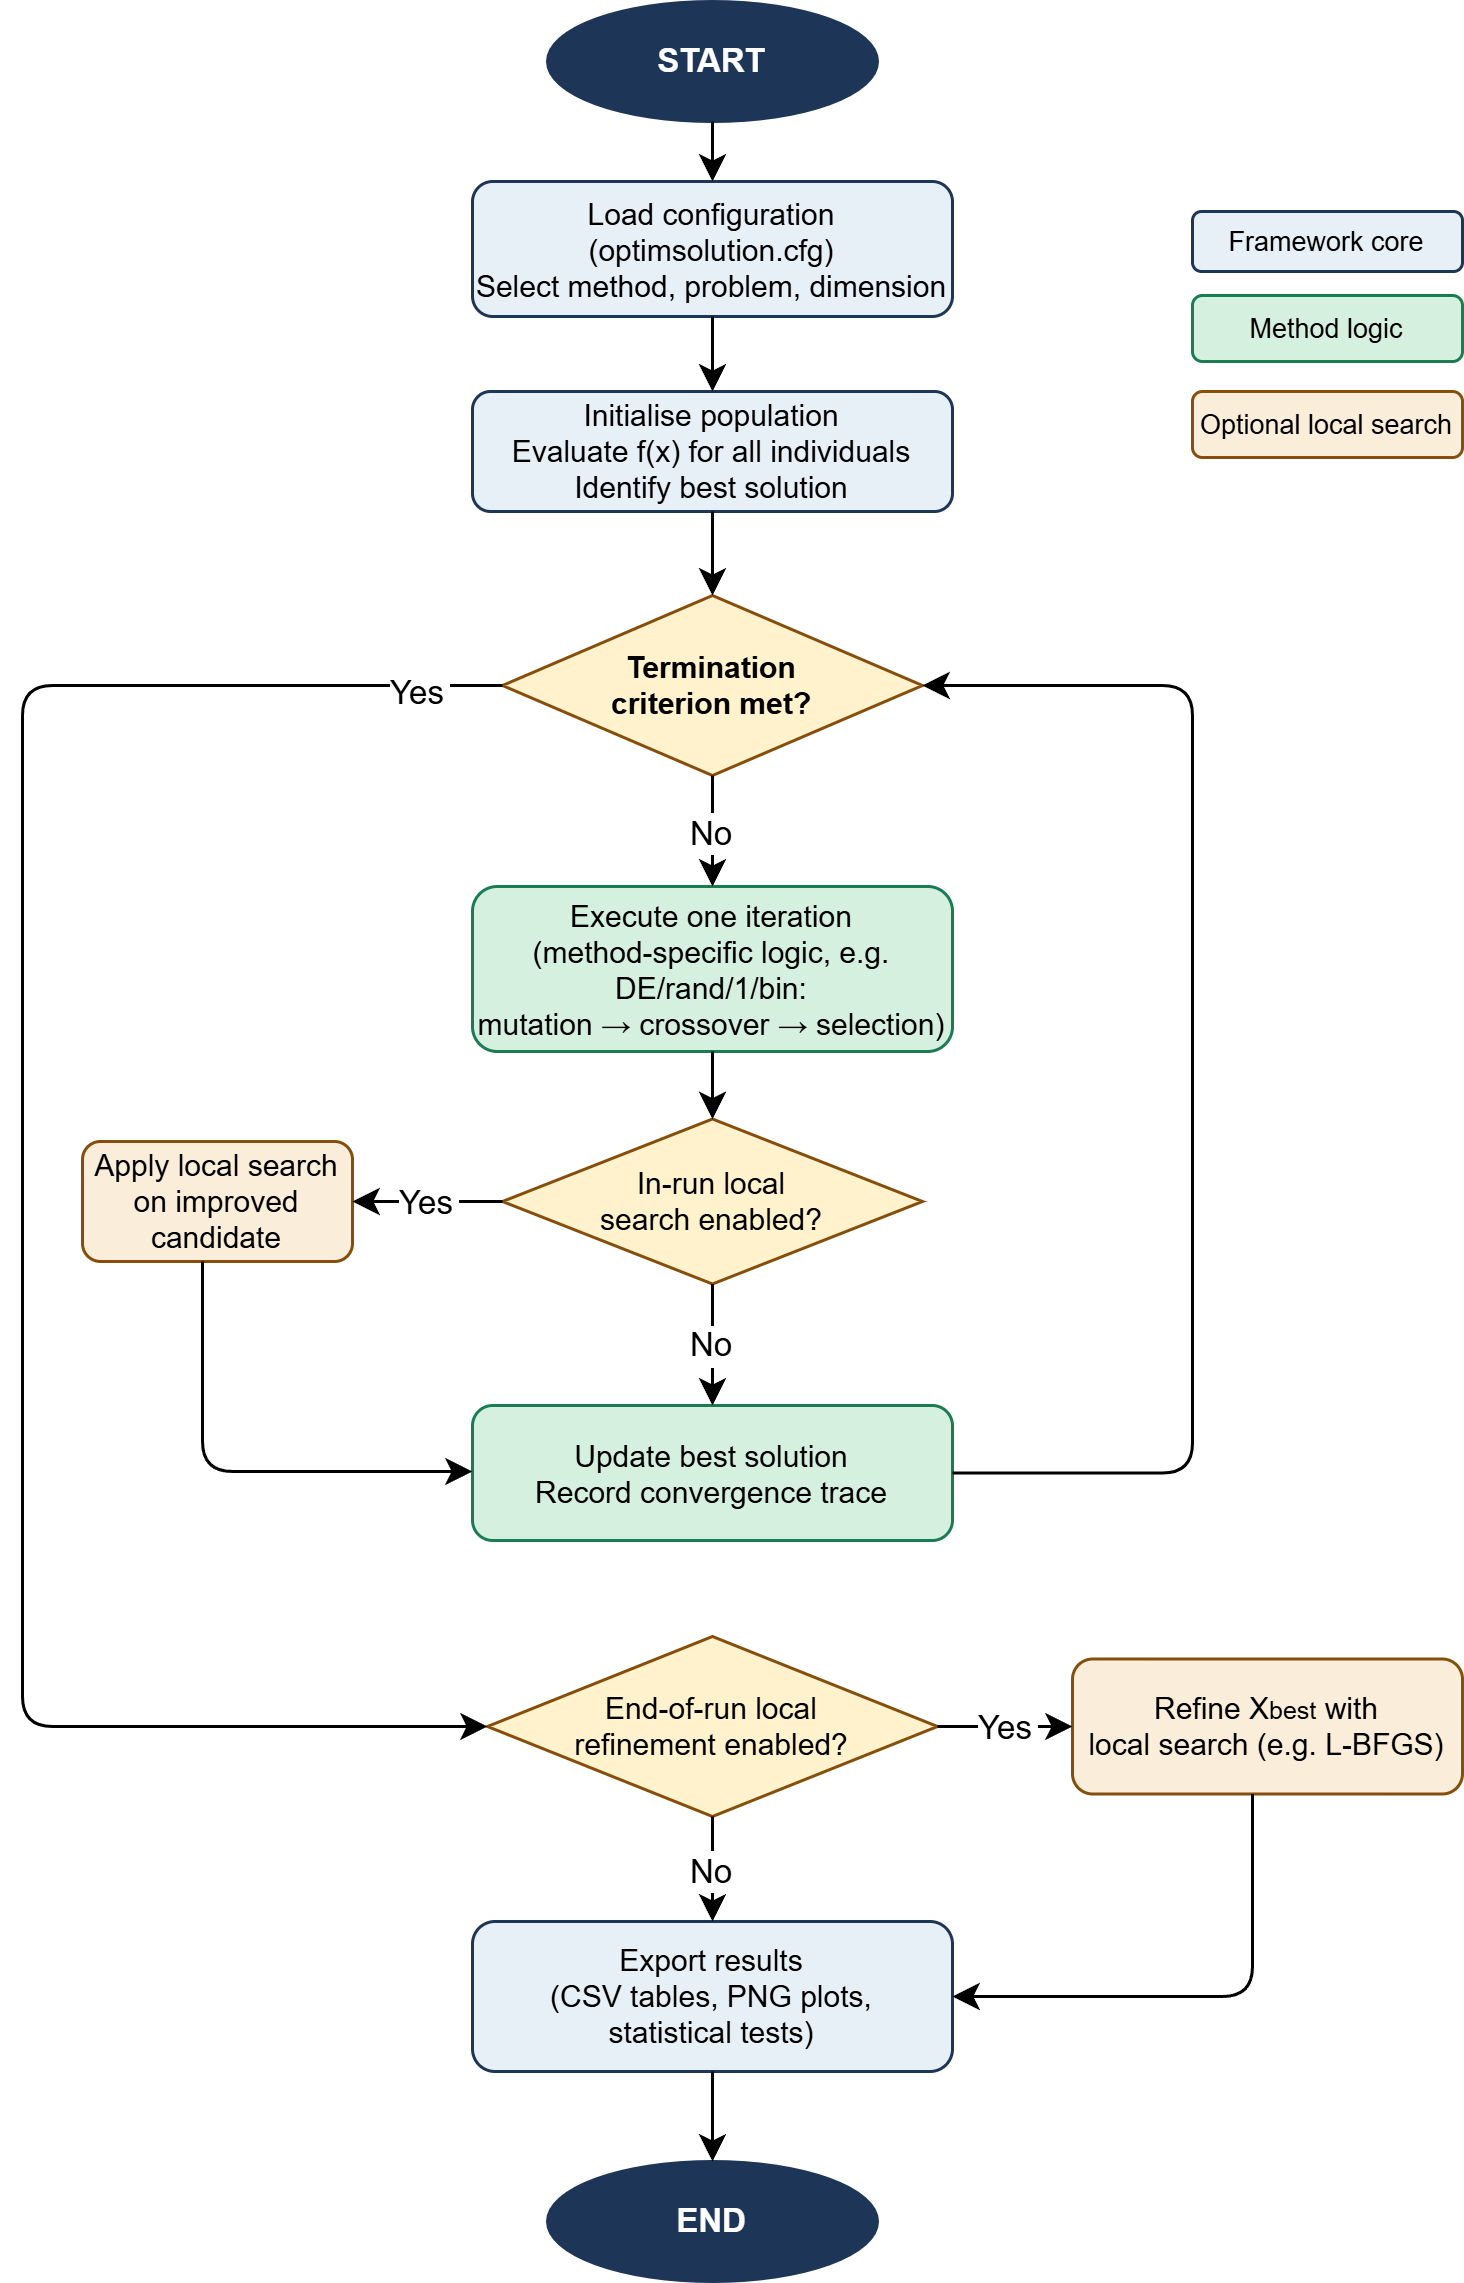
\includegraphics[scale=0.6]{optimsolution_flowchart}
\par\end{centering}
\caption{General execution flow of the OptimSolution framework. Blue: framework
core, green: method-specific logic, orange: optional local search
stages.\label{fig:flow}}
\end{figure}

Figure \ref{fig:flow} presents the general execution flow of OptimSolution.
Upon loading the configuration file, the framework initialises the
population and evaluates the objective function for all individuals.
The main loop iterates until a termination criterion is satisfied
maximum function evaluations, maximum iterations, or a convergence-based
stopping rule. Within each iteration, the method-specific optimization
logic is executed (for example, DE/rand/1/bin applies mutation, crossover,
and greedy selection), an optional in-run local search can be triggered
probabilistically on improved candidates. Upon termination, an optional
end-of-run local refinement polishes the best solution found before
results are exported as CSV files and PNG figures.

\subsection{Installation Procedure and Example Run\label{subsec:Installation-Procedure}}

The source code is openly available at \url{https://github.com/charilog/optimsolution}.
The software requires a C++17-compliant compiler and CMake \ensuremath{\ge}
3.16. The Qt6 library (https://qt.io) is additionally required for
compilation of the GUI target.

On Linux and macOS, after cloning the repository, the software is
built with the standard CMake workflow:

\begin{verbatim}
cmake -S . -B build -G Ninja \
  -DCMAKE_BUILD_TYPE=Release \
  -DCMAKE_PROJECT_INCLUDE=cmake/optimsolution_gui.cmake

cmake --build build --target optimsolution_gui
cmake --build build --target optimsolution

./build/optimsolution_gui
./build/optimsolution arq tersoffc
\end{verbatim}

Both the CLI executable (optimsolution) and the GUI application are
produced in the build directory.

On Windows, the same CMake procedure applies when Qt6 and a compatible
compiler (MSVC or MinGW) are available. 

\begin{verbatim}
cmake -S . -B build -G "Visual Studio 17 2022" -A x64 `
  "-DCMAKE_PROJECT_INCLUDE:FILEPATH=$PWD/cmake/optimsolution_gui.cmake" `
  "-DCMAKE_PREFIX_PATH=C:\Qt\6.10.1\msvc2022_64"

cmake --build build --config Release --target optimsolution_gui
cmake --build build --config Release --target optimsolution

& "C:\Qt\6.10.1\msvc2022_64\bin\windeployqt.exe" `
  --no-translations --compiler-runtime `
  ".\build\Release\optimsolution_gui.exe"
\end{verbatim}

Alternatively, a pre-compiled installer (OptimSolution.exe) is provided
in the repository, which installs the GUI application without requiring
the Qt library or a build toolchain.

\subsection{Extensibility Mechanism\label{subsec:Extensibility-Mechanism}}

A central design objective of OptimSolution is the ability to register
new optimization methods and new benchmark problems without modifying
the framework core and without requiring the user to interact with
the build system manually. This is achieved through a GUI-driven code
generation and build pipeline implemented in the CodeGenDialog module.

To add a new optimization method, the user invokes the New Method
wizard from within the GUI. The wizard collects the method's short
name, full name, C++ class name, and the definitions of its configurable
parameters (name, type, default value, and description). It then automatically
generates a conforming .h/.cpp skeleton, patches factory.cpp to register
the new method under its short name, and updates CMakeLists.txt to
include the new source file. The generated source files are immediately
opened in an integrated Code Editor dialog, where the user implements
the algorithm logic. A one-click Build button invokes the CMake build
pipeline from within the GUI and streams the compiler output to a
log panel. An equivalent New Problem wizard handles the registration
of new benchmark problems, additionally allowing the user to specify
dimensionality constraints, search-space bounds, and the known global
optimum value where available. Registered methods and problems can
equally be removed through a Delete dialog, which reverses the factory
and CMake patches and deletes the corresponding source files. The
complete extensibility workflow from specification to compilation
is thus contained within the GUI and requires no manual editing of
build or registration files.

\subsection{Additional Framework Features}

Termination criteria. OptimSolution provides ten configurable stopping
rules, selectable through the configuration file. In addition to the
standard maxevals (maximum function evaluations) and maxiters (maximum
iterations) criteria, the framework implements the convergence-based
rules bss, wss, tss, boss, srs, and irs, originally introduced and
validated in \citep{stop}, together with the doublebox criterion
and an all rule that triggers termination as a logical disjunction
of all active criteria halting execution as soon as any individual
rule is satisfied. This composite stopping mechanism ensures an adaptive
balance between convergence speed and solution accuracy across problem
instances of varying difficulty.

Population initialisation strategies. The initialisation of the population
is a critical factor affecting both the diversity of the initial search
and the ultimate convergence behaviour of metaheuristic algorithms
\citep{distribution}. OptimSolution supports eleven initialisation
distributions, selectable per experiment: uniform random sampling,
normal, Cauchy, Laplace, log-normal, exponential, Beta, and Lévy distributions,
as well as three structured strategies Latin Hypercube Sampling (LHS)
\citep{McKay}, Halton low-discrepancy sequences, and oppositional
initialisation. The k-means-based intelligent initialisation strategy
proposed in \citep{distribution} is also available, which uses a
clustering-driven approach to generate initial estimates more closely
aligned with the problem structure, thereby reducing the risk of premature
convergence.

Parallel methods. OptimSolution includes natively parallel optimization
methods that exploit multi-core architectures via OpenMP. The parallel
Genetic Algorithm (PGA) \citep{pga} maintains a set of autonomous
island subpopulations that periodically exchange their best solutions,
combining the global exploration capabilities of the island model
with the convergence guarantees of periodic migration. The Parallel
Smell Agent optimization (PSAO) \citep{psao} extends the single-population
SAO \citep{sao} with dynamic collaboration mechanisms and intelligent
solution dispersal among subpopulations, accelerating global exploration
while preventing premature convergence to local minima. Both methods
are configurable through the standard configuration file and are subject
to the same termination and initialisation options as all other framework
methods.

\section{Execution Modes and Analysis Features\label{sec:ExecutionModes}}

\subsection{Single Mode\label{subsec:Single-Mode}}

Single mode executes a selected optimization method on a selected
problem for a configurable number of independent runs. The user specifies
the method, problem, and problem dimensionality, all remaining parameters
population size, maximum function evaluations, number of runs, success
tolerance, local search settings, and output options are read from
a configuration file (optimsolution.cfg) shared between the CLI and
the GUI. Each independent run is initialised with a distinct random
seed derived from a common base seed, ensuring reproducibility while
preserving stochastic diversity. At each run, the framework records
the best objective function value as a function of function evaluations,
producing a convergence trajectory. In the convergence plot, each
line of the same colour corresponds to one independent run, the bundle
of lines collectively characterises both the reliability of the method
the consistency of its convergence behaviour across repeated trials
and its validity whether it systematically locates solutions of comparable
quality, ideally close to the known global optimum. Upon completion,
descriptive statistics across all runs best, worst, mean, standard
deviation, and success rate are reported and optionally exported as
CSV. A convergence curve plot and a box-plot of the final solution
values are generated and exportable as PNG.

Single mode additionally supports complexity analysis through two
overlay options available in both the GUI and the CLI. The first option
overlays convergence curves across a set of user-defined dimensionalities
for a fixed method-problem pair, characterising the scalability of
the method as problem size grows. The second option overlays convergence
curves across a set of methods for a fixed problem and dimensionality,
producing a difficulty profile of the problem as seen by a method
portfolio. Figure \ref{fig:complexity} illustrates an example of
the first option: ABC applied to the Ackley function across dimensions
D = 6, 12, 18, and 24, where each colour corresponds to a different
dimensionality and the spread of same-colour lines reflects run-to-run
variability at that dimension.

\begin{figure}[H]
\begin{centering}
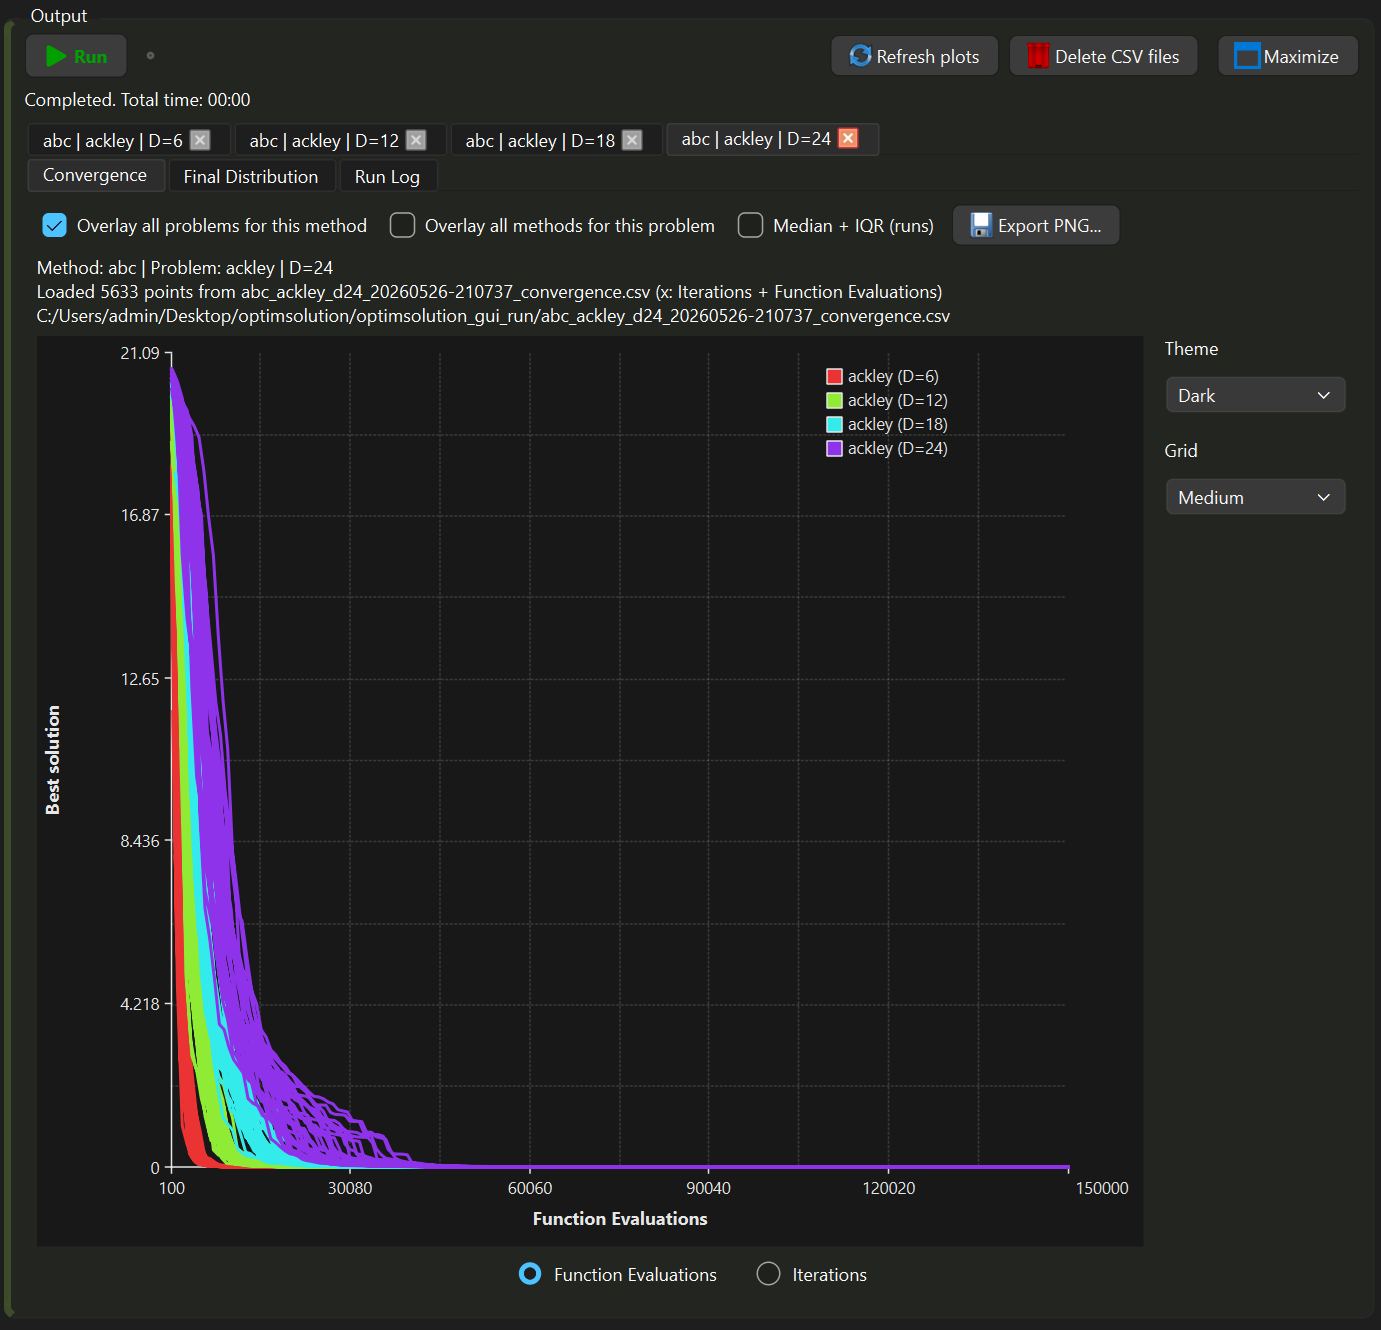
\includegraphics[scale=0.35]{complexity}
\par\end{centering}
\caption{Convergence curves of ABC on the Ackley function for D = 6, 12, 18,
and 24. Each colour denotes a dimensionality, same-colour lines are
the 30 independent runs, reflecting method reliability and validity
across problem scales\label{fig:complexity}}

\end{figure}


\subsection{Batch Mode\label{subsec:Batch-Mode}}

Batch mode automates the systematic evaluation of a user-defined set
of methods across a user-defined set of problems. The framework executes
every method-problem combination for the number of independent runs
specified in the configuration file, processing all jobs sequentially
and reporting progress in real time. Figure \ref{fig:batch1} illustrates
an in-progress batch experiment comparing jSO and mLSHADE-RL on the
Economic Load Dispatch problems eld1, eld2, and eld3 \citep{Das}
at dimensions D = 6, 13, and 15 respectively. The results table displays,
for each method-problem pair, the best value found across all runs,
the mean, the success rate, the standard deviation, and the mean wall-clock
time per run, enabling a direct quantitative comparison.

\begin{figure}[H]
\begin{centering}
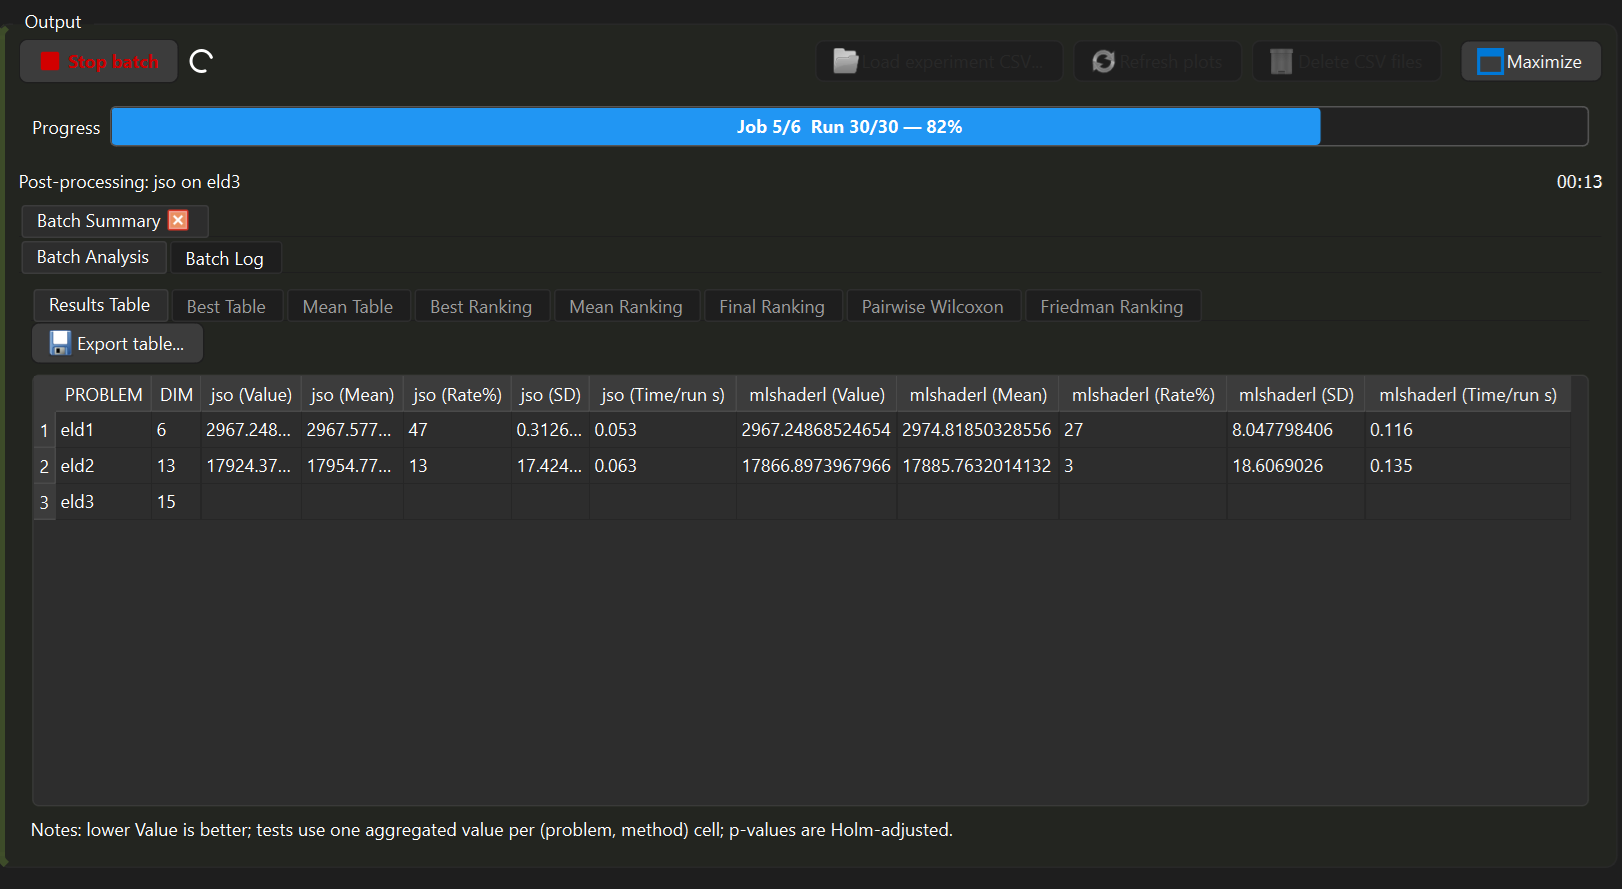
\includegraphics[scale=0.3]{batch1}
\par\end{centering}
\caption{Batch mode results table during execution (Job 5/6, Run 30/30) comparing
jSO and mLSHADE-RL on eld1, eld2, and eld3, reporting best value,
mean, success rate, standard deviation, and time per run for each
method--problem pair\label{fig:batch1}}
\end{figure}

Upon completion, the Batch Analysis panel organises the results across
eight views: Results Table, Best Table, Mean Table, Best Ranking,
Mean Ranking, Final Ranking, Pairwise Wilcoxon, and Friedman Ranking.
Figure \ref{fig:batch2} shows the Pairwise Wilcoxon view for the
same experiment: box plots of the final best-value distributions are
displayed for each method, aggregated across all three problems, with
Holm-adjusted p-values annotated for each comparison. In this example,
the comparison between jSO and mLSHADE-RL yields $p_{adj}$ = 0.371,
indicating no statistically significant difference at $\alpha$ =
0.05. All tables and plots are exportable as CSV and PNG respectively.

\begin{figure}[H]
\begin{centering}
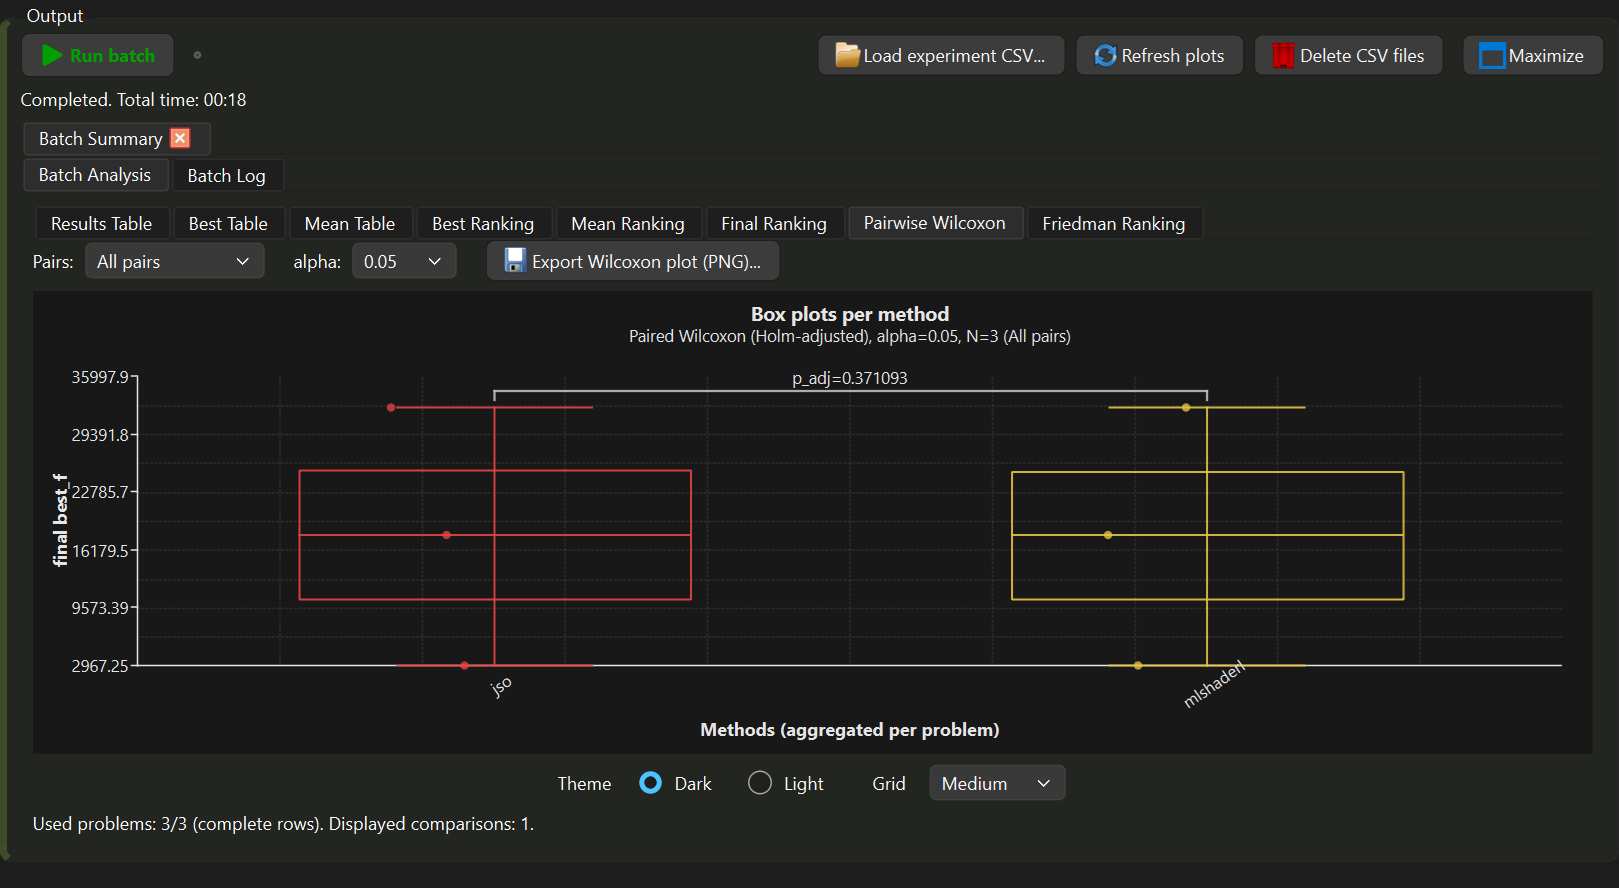
\includegraphics[scale=0.3]{batch2}
\par\end{centering}
\caption{Pairwise Wilcoxon box plots for jSO vs. mLSHADE-RL aggregated over
three Economic Load Dispatch problems (N = 3), with Holm-adjusted
p-value ($p_{adj}$ = 0.371, $\alpha$ = 0.05), indicating no statistically
significant difference between the two methods\label{fig:batch2}}
\end{figure}


\subsection{Method and Problem Sensitivity Analysis\label{subsec:Sensitivity-Analysis}}

OptimSolution provides two complementary sensitivity analysis modes,
accessible through dedicated run-mode selections in both the GUI and
the CLI.

Method sensitivity analysis examines how variations in an algorithm's
own hyper-parameters affect its performance on a selected set of problems.
The user specifies the parameter of interest and the discrete values
to evaluate through the Sensitivity panel of the Settings window,
the framework then executes the method for each parameter value across
all selected problems for the configured number of independent runs,
and produces a Results table reporting for each parameter value the
mean best objective value, standard deviation, minimum, maximum, main
effect, rank, and number of runs. Figure \ref{fig:sen1} illustrates
an example in which the parameter delta of ARQ2 \citep{ARQ,ARQ2}
is swept over the values \{0.1, 0.3, 0.5, 0.7, 0.9\} on the Economic
Load Dispatch problems eld1 (D = 6) and eld2 (D = 13). The table in
Figure \ref{fig:sen1} highlights in bold the top-ranked configuration,
here delta = 0.3 achieves the lowest mean best value on eld2 (mean
$best_{f}$ = 17876.697, rank 1). Figure \ref{fig:sen2} shows the
corresponding bar chart for eld2, where each bar represents the mean
best value with a 95\% confidence interval and the green bar identifies
the optimal parameter value, allowing the practitioner to distinguish
robust from critical parameter regions.

\begin{figure}[H]
\begin{centering}
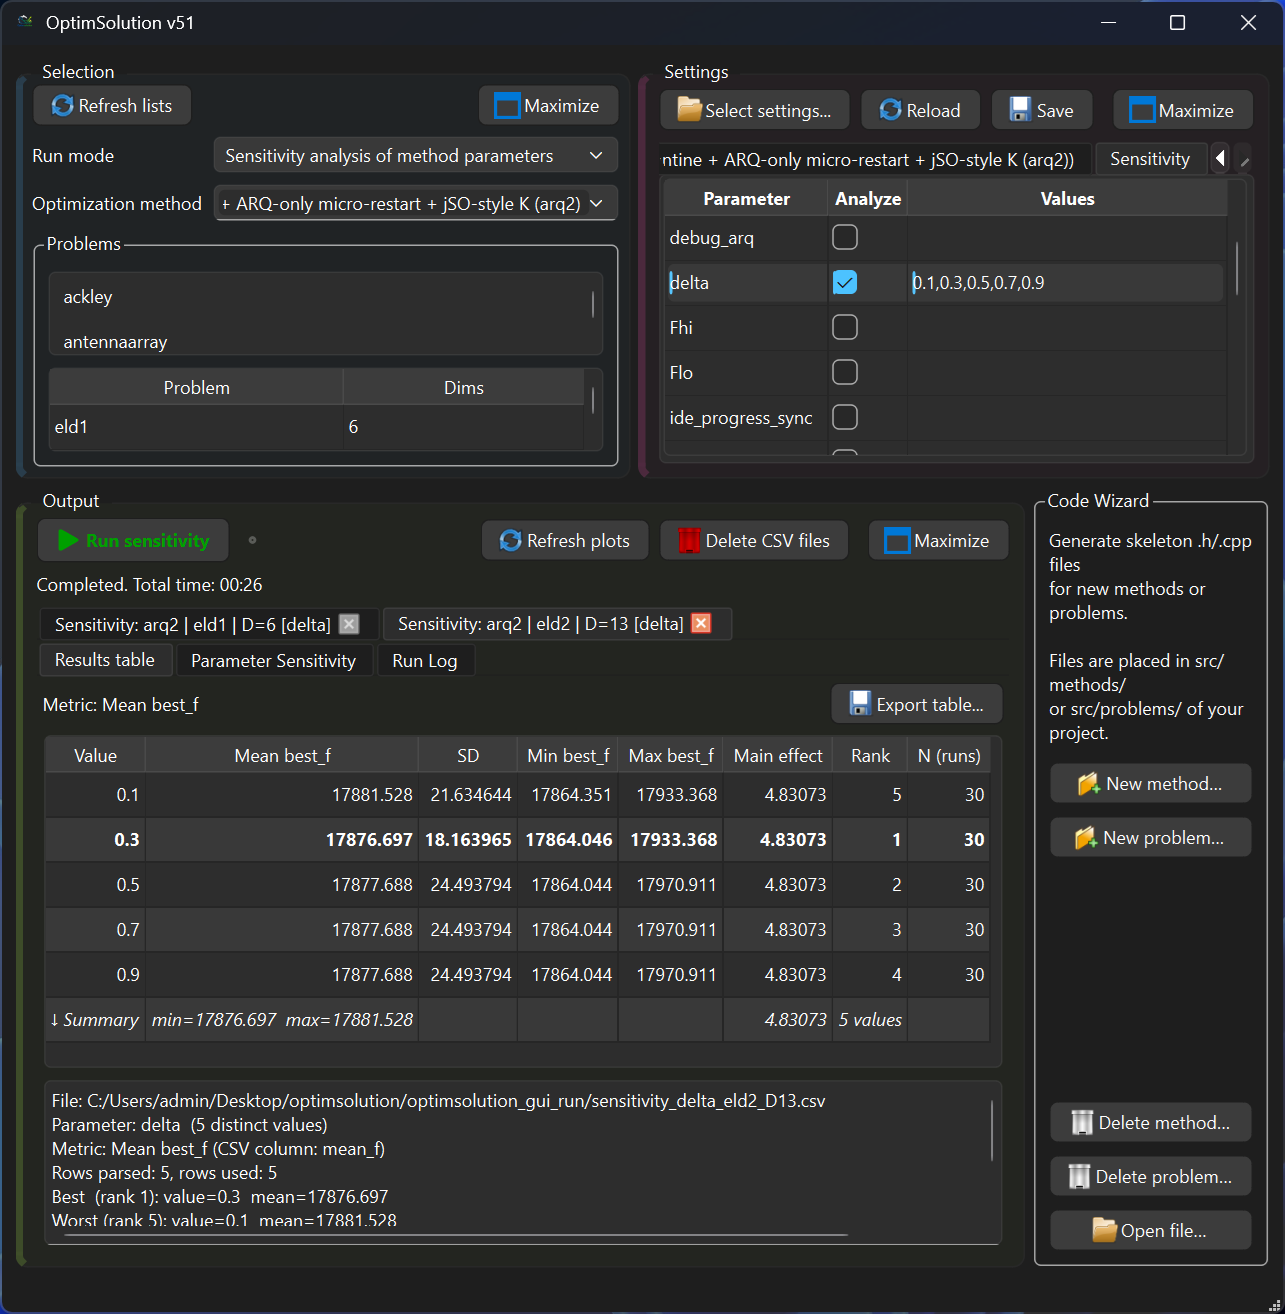
\includegraphics[scale=0.3]{sen1}
\par\end{centering}
\caption{Method sensitivity GUI: ARQ2 parameter delta \ensuremath{\in} \{0.1,
0.3, 0.5, 0.7, 0.9\} on eld1 (D = 6) and eld2 (D = 13)\label{fig:sen1}}
\end{figure}

\begin{figure}[H]
\begin{centering}
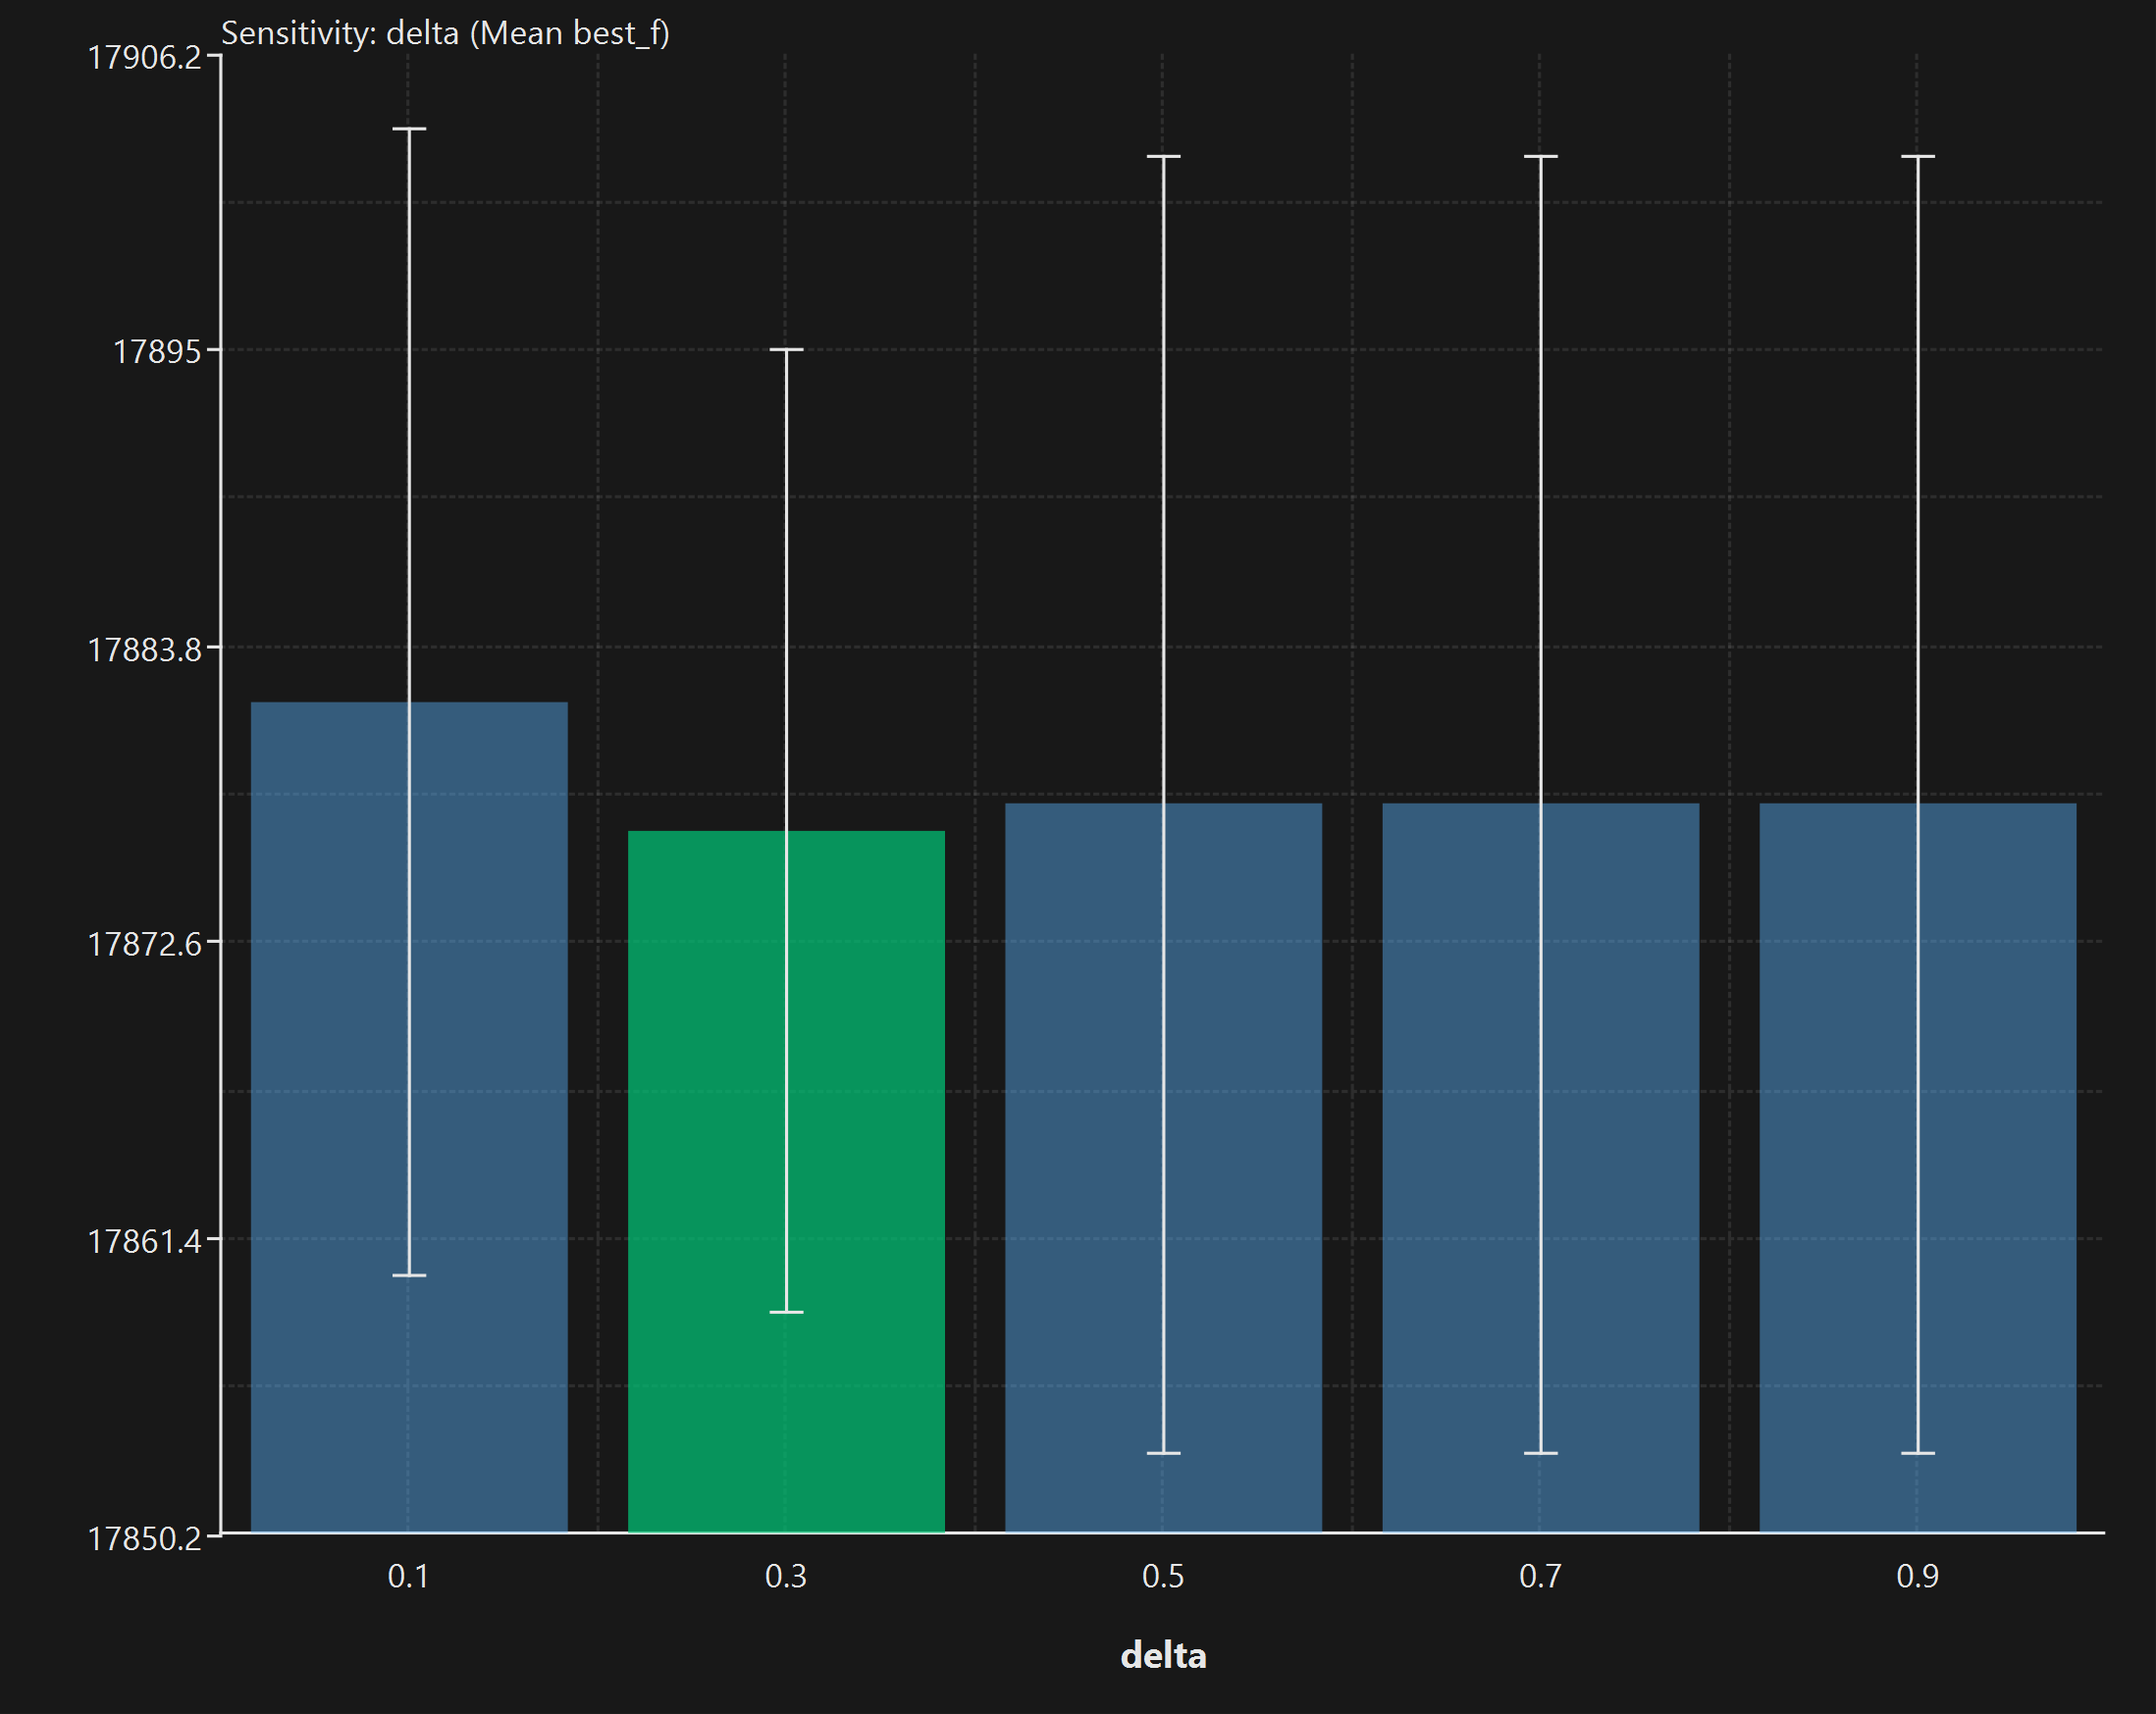
\includegraphics[scale=0.55]{sen2}
\par\end{centering}
\caption{Mean best\_f with 95\% confidence intervals per value of delta on
eld2 (D = 13). Green bar: optimal setting (delta = 0.3)\label{fig:sen2}}
\end{figure}

Problem sensitivity analysis examines how variations in a problem's
own defining parameters affect instance difficulty and the relative
performance of a selected method. The user selects a problem, a method,
and one or more problem parameters to sweep, the framework applies
the method to each resulting problem instance and reports the same
set of metrics. Figure \ref{fig:sen3} shows an example in which ARQ2
is applied to the weatherirrigation problem at D = 30, sweeping the
parameter $osc_{fre\text{\_}base}$ over the values \{0.19, 0.20,
0.21, 0.22, 0.23, 0.24\}. The best-performing problem configuration
is $osc_{fre\text{\_}base}$ = 0.24 (mean $best_{f}$ = 2738.37, rank
1), while the most difficult instance for this method is $osc_{fre\text{\_}base}$
= 0.19 (mean $best_{f}$ = 2757.60, rank 6). Figure \ref{fig:sen4}
shows the corresponding bar chart, where the green bar identifies
the parameter value that minimises the mean objective value. All results
are exported as CSV and PNG.

\begin{figure}[H]
\begin{centering}
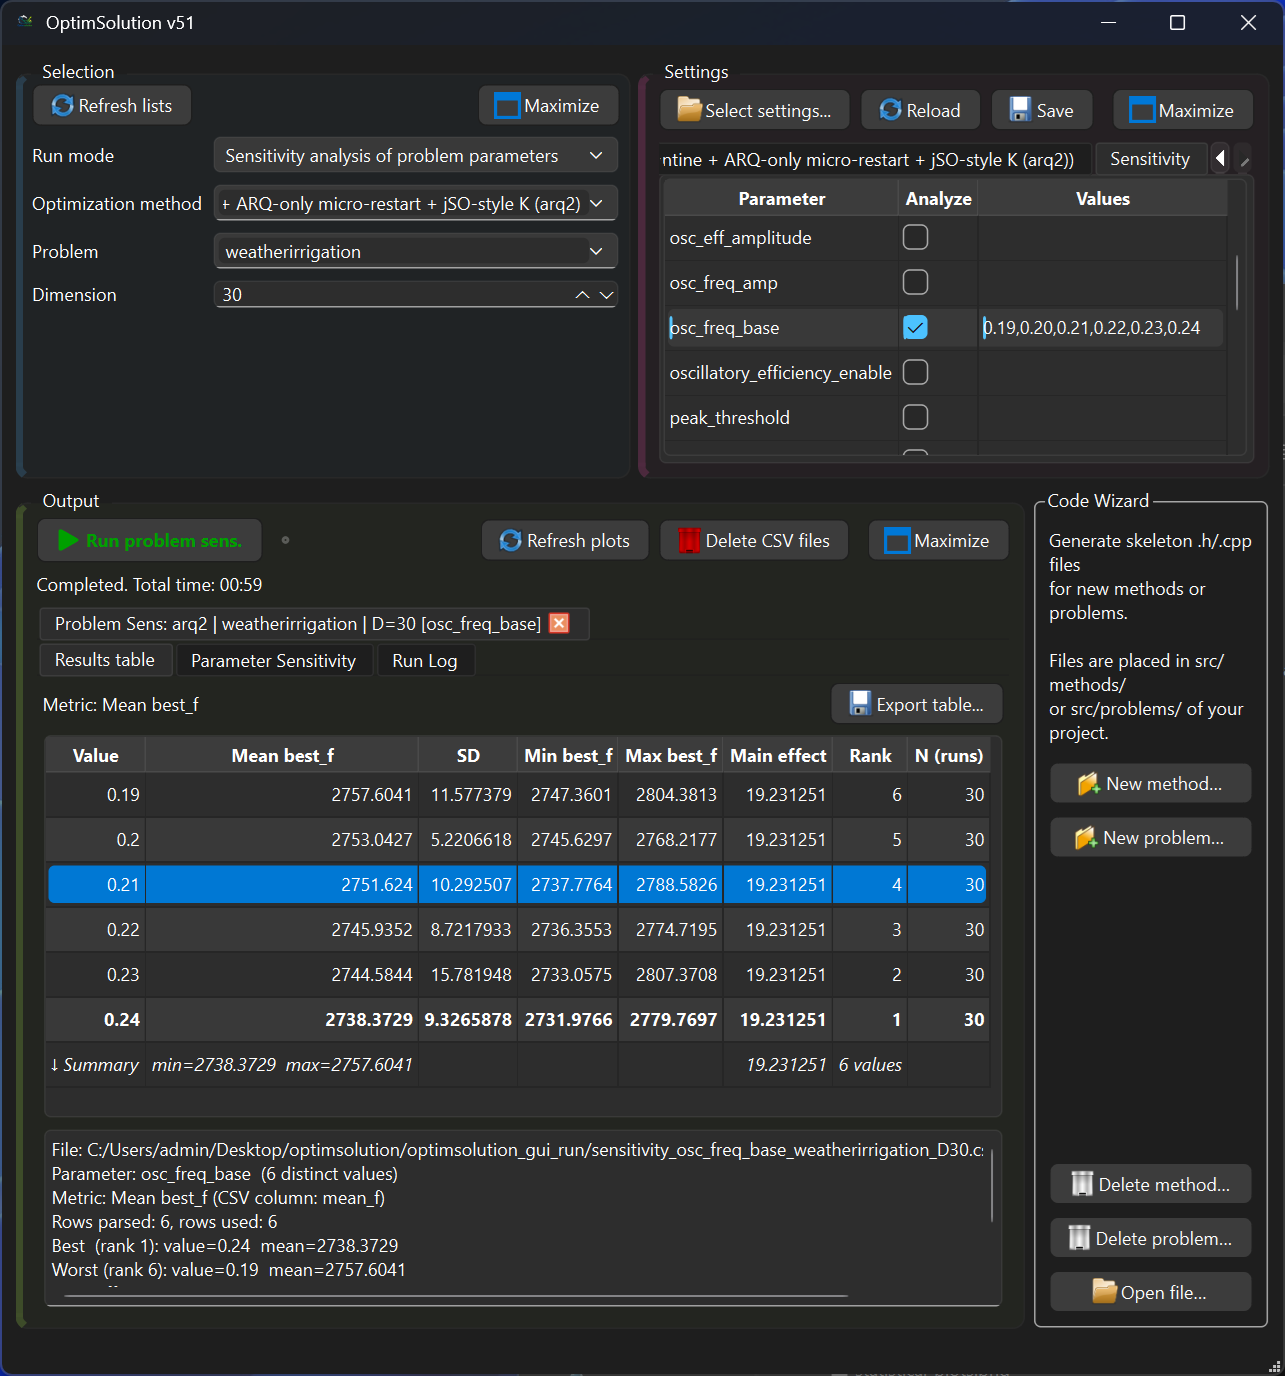
\includegraphics[scale=0.3]{sen3}
\par\end{centering}
\caption{Problem sensitivity GUI: ARQ2 on weatherirrigation (D = 30) with $osc_{fre\text{\_}base}$
\ensuremath{\in} \{0.19, \ldots , 0.24\}\label{fig:sen3}}
\end{figure}

\begin{figure}[H]
\begin{centering}
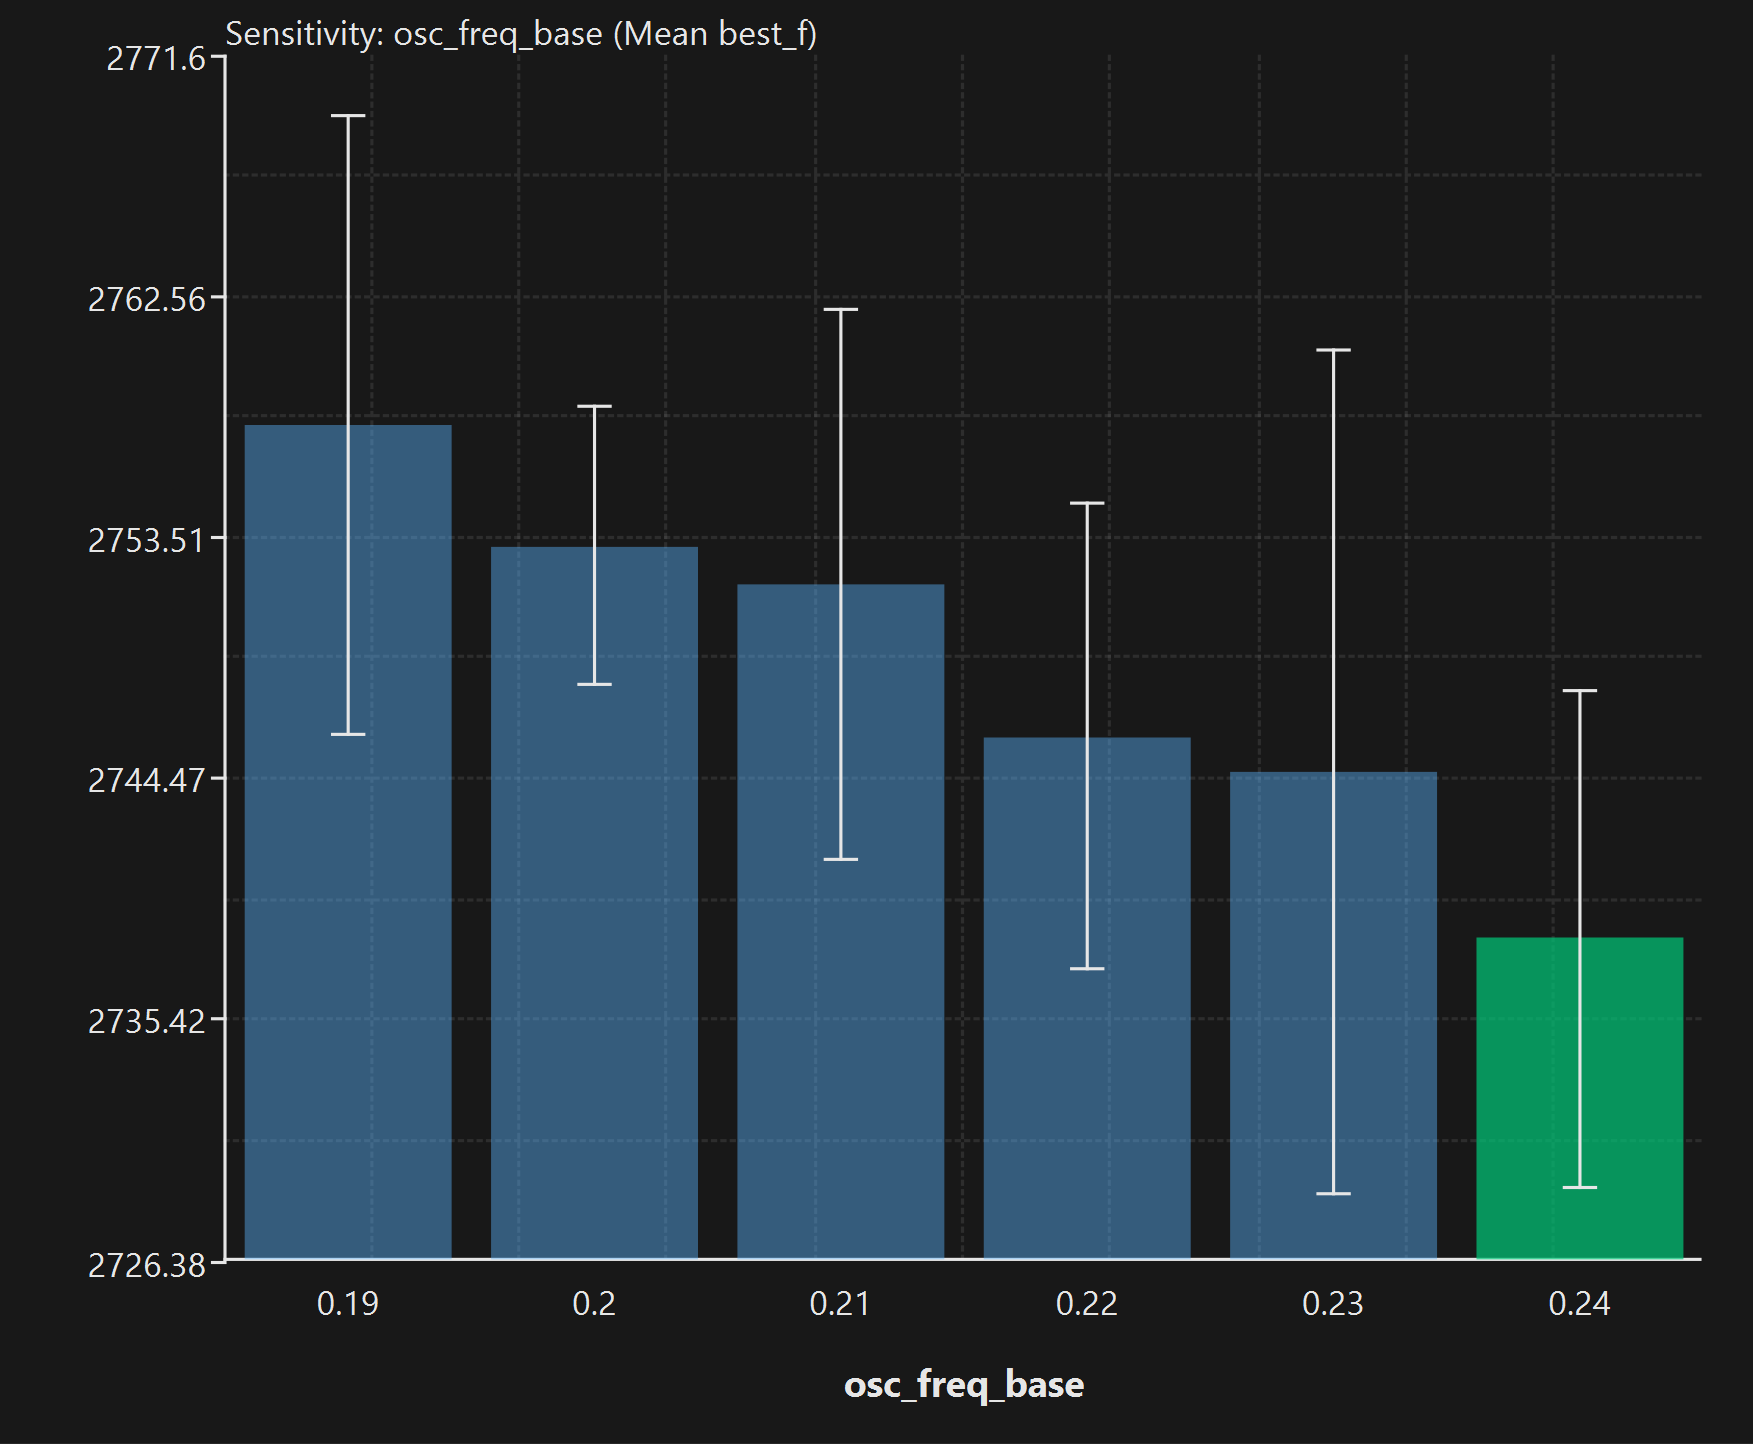
\includegraphics[scale=0.7]{sen4}
\par\end{centering}
\caption{Mean best\_f with 95\% confidence intervals per value of $osc_{fre\text{\_}base}$
on weatherirrigation (D = 30). Green bar: optimal setting ( $osc_{fre\text{\_}base}$=
0.24)\label{fig:sen4}}
\end{figure}


\subsection{GUI Execution Performance\label{subsec:GUIPerformance}}

Although the GUI and the CLI share an identical computational core,
the GUI achieves substantially lower wall-clock execution times on
multi-run experiments. Figures \ref{fig:cli} and \ref{fig:gui} document
a direct comparison: jSO was applied to the six-element circular antenna
array synthesis problem \citep{Das} (D = 12) for 30 independent runs
under identical configuration. As reported in the CLI summary (Figure
9), the mean time per run was 8.38 seconds, yielding a total wall-clock
time of 251.37 seconds, with a best objective value of 0.00680964
and a 100\% success rate across all 30 runs. The GUI completed the
same experiment in 125 seconds (Figure \ref{fig:gui}), delivering
an identical best objective value and convergence profile a speedup
factor of approximately 2.0\texttimes{} with no loss in solution quality.

\begin{figure}[H]
\begin{centering}
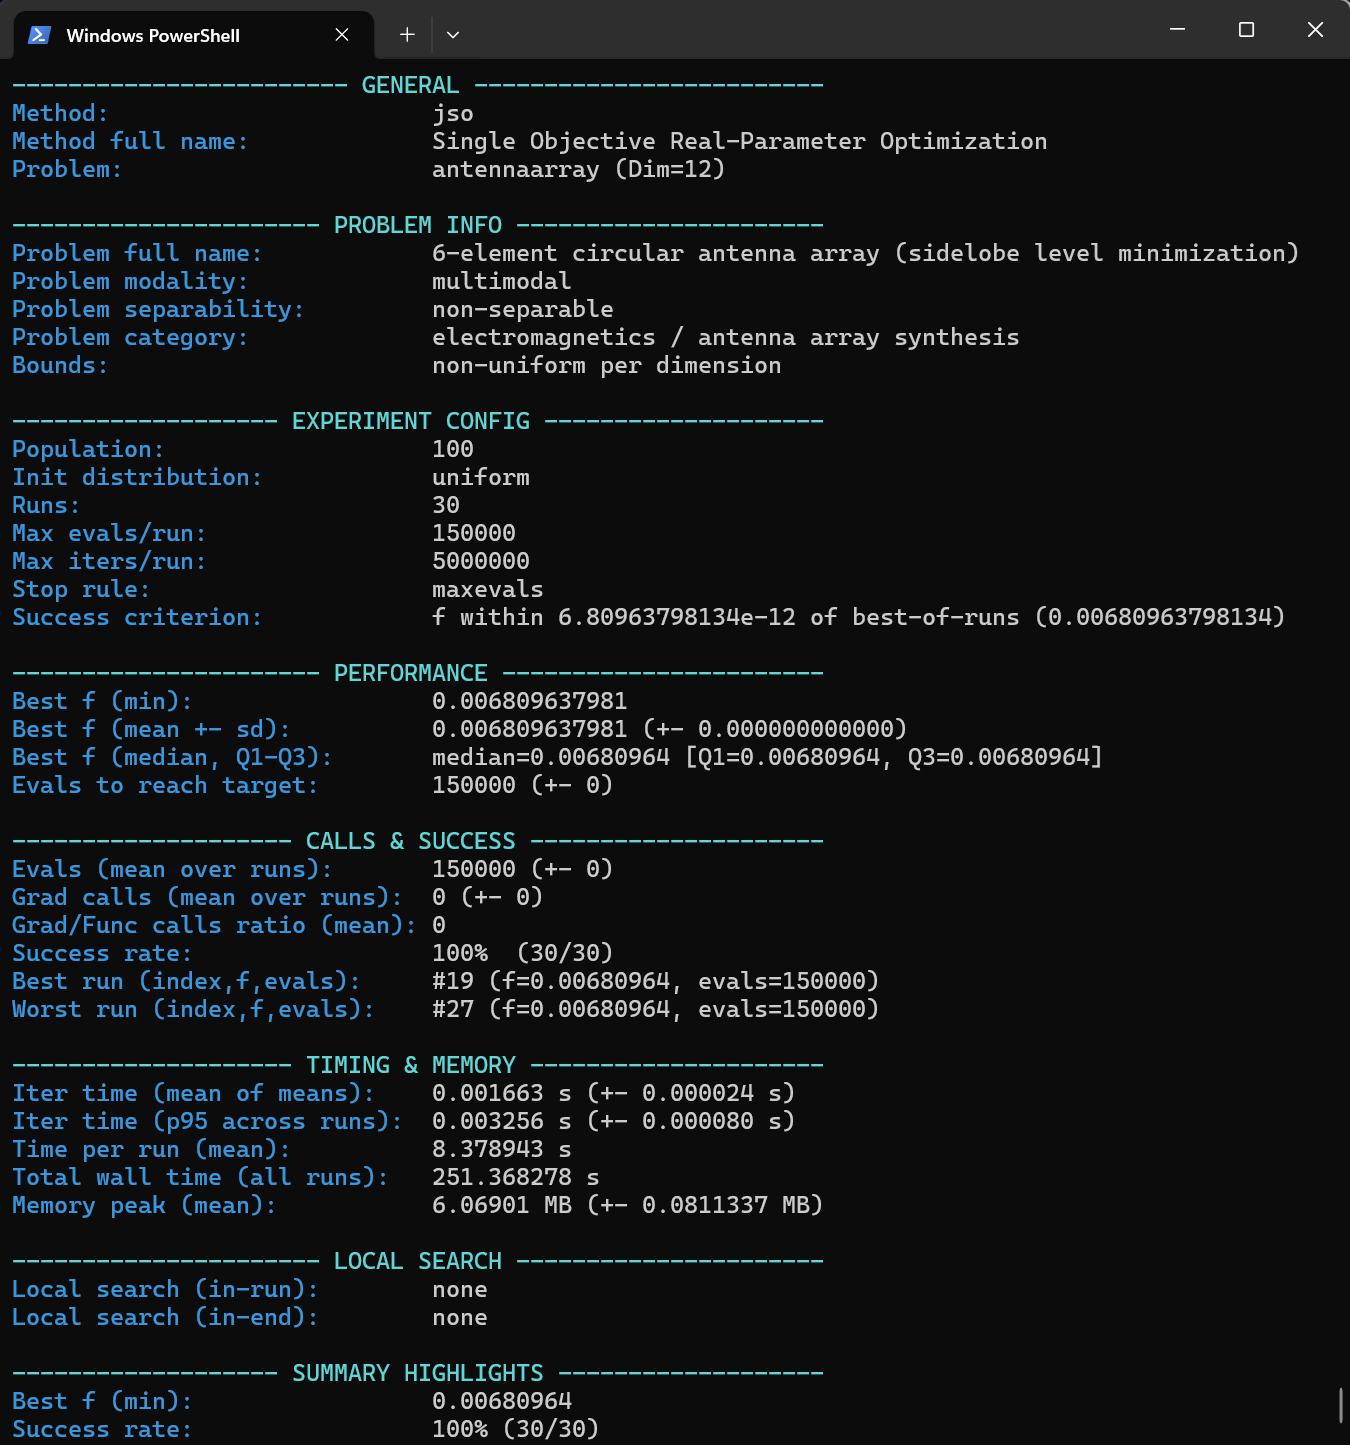
\includegraphics[scale=0.35]{cli}
\par\end{centering}
\caption{CLI summary output for jSO on the antenna array synthesis problem
(D = 12, 30 runs): best f = 0.00680964, success rate 100\%, mean time
per run 8.38 s, total wall time 251.37 s.\label{fig:cli}}
\end{figure}

\begin{figure}[H]
\begin{centering}
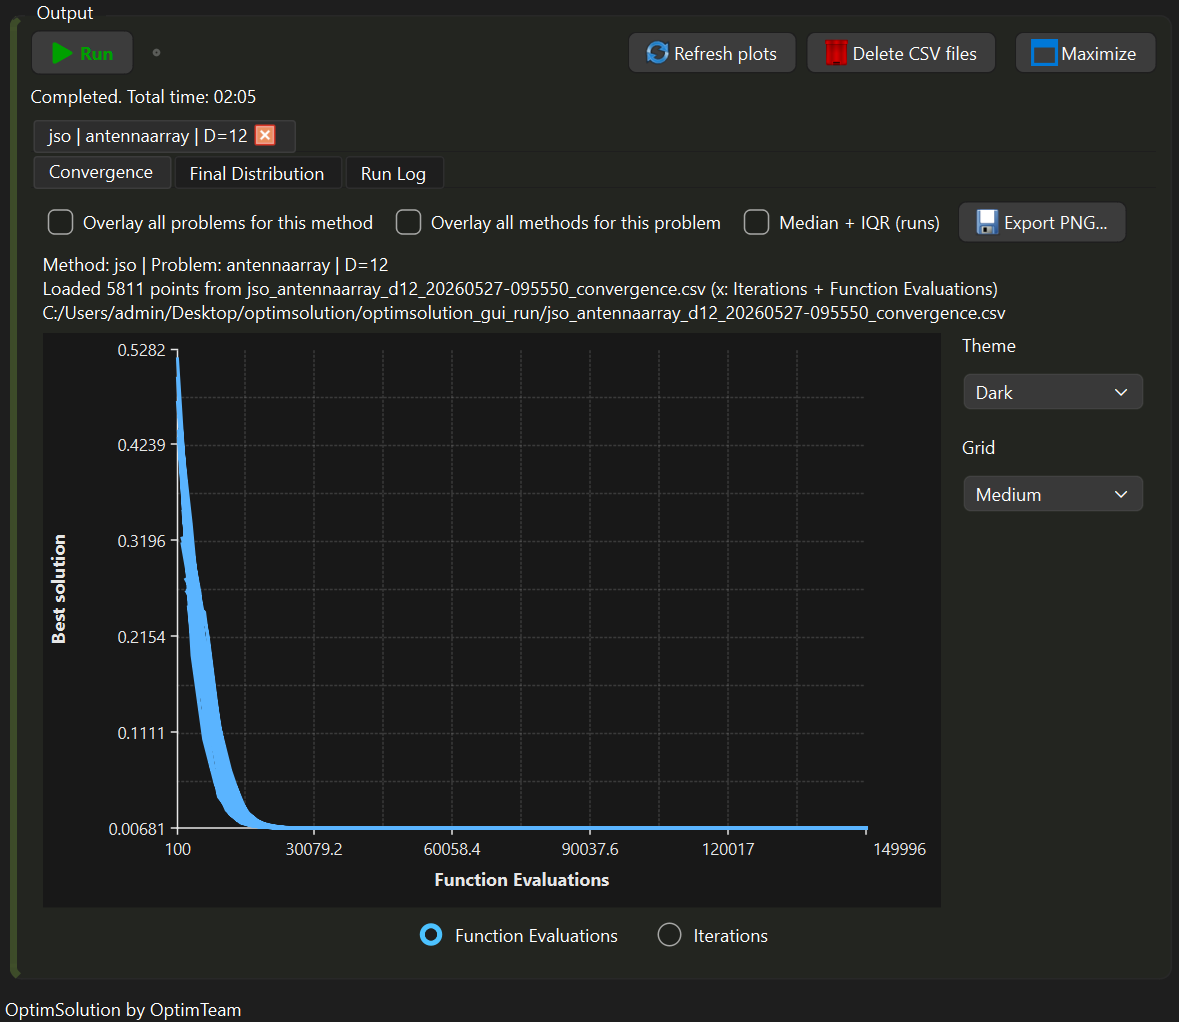
\includegraphics[scale=0.35]{gui}
\par\end{centering}
\caption{GUI output for the same experiment: convergence curves of the 30 independent
runs and total elapsed time of 125 s (02:05), confirming identical
solution quality at half the wall-clock time.\label{fig:gui}}
\end{figure}

This acceleration arises from three optimization strategies implemented
in the GUI layer. First, process output is not rendered in real time,
it is accumulated in an internal buffer and flushed to the log panel
at fixed intervals, preventing the graphical event loop from processing
thousands of individual rendering events per second. Second, at each
flush only a filtered subset of output lines is displayed, further
reducing the UI update cost during long runs. Third, once a run completes,
result parsing and statistical aggregation are performed concurrently
on a background thread while the next run is already launching in
the foreground, effectively pipelining computation and I/O. Together,
these mechanisms decouple the graphical interface from the computational
workload, allowing the GUI to deliver faster end-to-end experiment
completion times than an equivalent sequential CLI workflow.

\section{Conclusions\label{sec:conclusions}}

This paper presented OptimSolution, an open-source, cross-platform
framework for the systematic benchmarking and multi-faceted analysis
of continuous optimization methods. The framework is operable via
both a Qt-based GUI and a CLI, runs natively on Linux, Windows, and
macOS, and provides a unified configuration layer that guarantees
identical experimental conditions across both interfaces. Four execution
modes Single, Batch, Method Sensitivity Analysis, and Problem Sensitivity
Analysis together with a Complexity Analysis module, cover the full
spectrum of evaluation tasks required in modern metaheuristic research.
Embedded non-parametric statistical testing via Wilcoxon signed-rank
and Friedman tests with post-hoc Holm-adjusted pairwise comparisons,
rank plots, and box-plot visualisations provides publication-ready
statistical validation without reliance on external tools. The problem
layer comprises approximately 90 instances drawn from classical analytical
suites, the CEC 2022 benchmark suite, GKLS random function instances,
the complete CEC 2011 real-world problem suite, and original engineering
design problems. The method layer encompasses approximately 68 optimization
algorithms, ranging from foundational metaheuristics to state-of-the-art
competition variants. An in-GUI extensibility mechanism allows new
methods and problems to be registered, compiled, and activated without
any modification to the framework core, supporting rapid experimental
iteration. A comparative evaluation against nine existing frameworks
demonstrated that no alternative tool combines this feature set within
a single self-contained environment. 

Furthermore, an empirical timing comparison showed that the GUI achieves
a speedup of approximately 2\texttimes{} over an equivalent sequential
CLI workflow, attributable to buffered log rendering, output filtering,
and concurrent post-processing on a background thread. Several directions
present themselves as natural extensions of the current work. First,
support for constrained optimization including penalty-based, feasibility-rule,
and repair-operator approaches would substantially extend the applicability
of the framework to engineering design problems with explicit constraints.
Second, the integration of multi-objective optimization modes, with
Pareto front visualisation and hypervolume-based statistical comparison,
would broaden the framework's scope to a class of problems of growing
practical importance. Third, a Python API built on top of the existing
C++ core via a binding layer would make OptimSolution directly accessible
within Python-based research pipelines and machine learning workflows,
removing the current barrier for users who prefer scripted experimentation.
Fourth, parallel and distributed execution of independent runs for
example via OpenMP for shared-memory parallelism or MPI for cluster
environments would further reduce wall-clock time for large-scale
benchmarking studies involving many methods, problems, and dimensionalities.
Finally, the integration of automated hyperparameter tuning for the
registered methods, leveraging the existing sensitivity analysis infrastructure,
would provide a closed-loop optimization-of-optimization capability
directly within the framework.

\appendixtitles{no}

\begin{adjustwidth}{-\extralength}{0cm}{}


\reftitle{References}
\begin{thebibliography}{999}
\bibitem{Floudas}Floudas, C.A.; Pardalos, P.M. Encyclopedia of Optimization,
2nd ed.; Springer: New York, NY, USA, 2009.

\bibitem{Holland}Holland, J.H. Adaptation in Natural and Artificial
Systems; University of Michigan Press: Ann Arbor, MI, USA, 1975.

\bibitem{Kennedy}Kennedy, J.; Eberhart, R.C. Particle swarm optimization.
In Proc. IEEE Int. Conf. Neural Networks, Perth, Australia, 1995;
pp. 1942-1948. https://doi.org/10.1109/ICNN.1995.488968

\bibitem{Storn}Storn, R.; Price, K. Differential evolution - a simple
and efficient heuristic for global optimization over continuous spaces.
J. Glob. Optim. 1997, 11, 341-359. https://doi.org/10.1023/A:1008202821328

\bibitem{Beiranvand}Beiranvand, V.; Hare, W.; Lucet, Y. Best practices
for comparing optimization algorithms. Optim. Eng. 2017, 18, 815-848.
https://doi.org/10.1007/s11081-017-9366-1

\bibitem{Bartz-Beielstein}Bartz-Beielstein, T.; Doerr, C.; et al.
Benchmarking in Optimization: Best Practice and Open Issues. arXiv
2020, arXiv:2007.03488.

\bibitem{Kononova}Kononova, A.V.; et al. Assessing ranking and effectiveness
of evolutionary algorithm hyperparameters using global sensitivity
analysis methodologies. arXiv 2022, arXiv:2207.04820.

\bibitem{Hansen}Hansen, N.; Auger, A.; Ros, R.; Mersmann, O.; Tušar,
T.; Brockhoff, D. COCO: A platform for comparing continuous optimizers
in a black-box setting. Optimization Methods and Software 2021, 36,
114-144. https://doi.org/10.1080/10556788.2020.1808977

\bibitem{Doerr}Doerr, C.; Wang, H.; Ye, F.; van Rijn, S.; Bäck, T.
IOHprofiler: A benchmarking and profiling tool for iterative optimization
heuristics. arXiv 2019, arXiv:1810.05281. https://doi.org/10.48550/arXiv.1810.05281

\bibitem{Rapin}Rapin, J.; Teytaud, O. Nevergrad - A gradient-free
optimization platform. ACM SIGEVOlution 2021, 14, 8-15. \newline{https://doi.org/10.1145/3460310.3460312}

\bibitem{Blank}Blank, J.; Deb, K. pymoo: Multi-objective optimization
in Python. IEEE Access 2020, 8, 89497-89509. \newline{https://doi.org/10.1109/ACCESS.2020.2990567}

\bibitem{Van}Van Thieu, N.; Mirjalili, S. MEALPY: An open-source
library for latest meta-heuristic algorithms in Python. Journal of
Systems Architecture 2023, 139, 102871. https://doi.org/10.1016/j.sysarc.2023.102871

\bibitem{Vrban=00010Di=00010D}Vrbančič, G.; Brezočnik, L.; Mlakar,
U.; Fister, D.; Fister, I. NiaPy: Python microframework for building
nature-inspired algorithms. Journal of Open Source Software 2018,
3, 613. https://doi.org/10.21105/joss.00613

\bibitem{Van2}Van Thieu, N. Opfunu: An open-source Python library
for optimization benchmark functions. Journal of Open Research Software
2024. https://doi.org/10.5334/jors.508

\bibitem{Tsoulos}Tsoulos, I.G.; Tzallas, A.; Karvounis, E. GlobalOptimus:
An open-source optimization tool. Journal of Open Source Software
2025. https://doi.org/10.21105/joss.07584

\bibitem{Serr=0000E9}Serré, G.; Kalogeratos, A.; Vayatis, N. GLOBe:
A modular global optimization library. HAL Preprint 2026, hal-05623801.
https://hal.science/hal-05623801v1

\bibitem{Wilcoxon}Wilcoxon, F. Individual comparisons by ranking
methods. Biometrics Bulletin 1945, 1, 80--83. https://doi.org/10.2307/3001968

\bibitem{Friedman}Friedman, M. The use of ranks to avoid the assumption
of normality implicit in the analysis of variance. Journal of the
American Statistical Association 1937, 32, 675--701. https://doi.org/10.2307/2279372

\bibitem{M=0000FChlenbein}Rastrigin, L.A. Systems of Extremal Control;
Nauka: Moscow, Russia, 1974.

\bibitem{Rosenbrock}Rosenbrock, H.H. An automatic method for finding
the greatest or least value of a function. The Computer Journal 1960,
3, 175--184. https://doi.org/10.1093/comjnl/3.3.175

\bibitem{Ackley}Ackley, D.H. A Connectionist Machine for Genetic
Hillclimbing; Kluwer Academic Publishers: Boston, MA, USA, 1987. https://doi.org/10.1007/978-1-4613-1997-9

\bibitem{Jamil}Jamil, M.; Yang, X.S. A literature survey of benchmark
functions for global optimization problems. International Journal
of Mathematical Modelling and Numerical optimization 2013, 4, 150--194.
https://doi.org/10.1504/IJMMNO.2013.055204

\bibitem{Kumar}Kumar, A.; Price, K.V.; Mohamed, A.W.; Hadi, A.A.;
Suganthan, P.N. Problem Definitions and Evaluation Criteria for the
CEC 2022 Special Session and Competition on Single Objective Bound
Constrained Numerical Optimization; Technical Report; Nanyang Technological
University: Singapore, 2021.

\bibitem{Gaviano}Gaviano, M.; Kvasov, D.E.; Lera, D.; Sergeyev, Y.D.
Algorithm 829: Software for generation of classes of test functions
with known local and global minima for global optimization. ACM Transactions
on Mathematical Software 2003, 29, 469--480. https://doi.org/10.1145/962437.962444

\bibitem{Das}Das, S.; Suganthan, P.N. Problem Definitions and Evaluation
Criteria for CEC 2011 Competition on Testing Evolutionary Algorithms
on Real World Optimization Problems; Technical Report; Jadavpur University
and Nanyang Technological University, 2011.

\bibitem{Hansen2}Hansen, N.; Ostermeier, A. Adapting arbitrary normal
mutation distributions in evolution strategies: The covariance matrix
adaptation. In Proceedings of the IEEE International Conference on
Evolutionary Computation, Nagoya, Japan, 1996; pp. 312--317. https://doi.org/10.1109/ICEC.1996.542381

\bibitem{Mirjalili}Mirjalili, S.; Lewis, A. The whale optimization
algorithm. Advances in Engineering Software 2016, 95, 51--67. \newline{https://doi.org/10.1016/j.advengsoft.2016.01.008} 

\bibitem{Mirjalili2}Mirjalili, S.; Mirjalili, S.M.; Lewis, A. Grey
wolf optimizer. Advances in Engineering Software 2014, 69, 46--61.
\newline{https://doi.org/10.1016/j.advengsoft.2013.12.007 } 

\bibitem{Karaboga}Karaboga, D. An Idea Based on Honey Bee Swarm for
Numerical Optimization; Technical Report TR06; Erciyes University:
Kayseri, Turkey, 2005.

\bibitem{Kirkpatrick}Kirkpatrick, S.; Gelatt, C.D.; Vecchi, M.P.
Optimization by simulated annealing. Science 1983, 220, 671--680.
\newline{https://doi.org/10.1126/science.220.4598.671} 

\bibitem{Socha}Socha, K.; Dorigo, M. Ant colony optimization for
continuous domains. European Journal of Operational Research 2008,
185, 1155--1173. https://doi.org/10.1016/j.ejor.2006.06.046

\bibitem{Rao}Rao, R.V.; Savsani, V.J.; Vakharia, D.P. Teaching--learning-based
optimization: A novel method for constrained mechanical design optimization
problems. Computer-Aided Design 2011, 43, 303--315. https://doi.org/10.1016/j.cad.2010.12.015

\bibitem{Rao2}Rao, R. Jaya: A simple and new optimization algorithm
for solving constrained and unconstrained optimization problems. International
Journal of Industrial Engineering Computations 2016, 7, 19--34. https://doi.org/10.5267/j.ijiec.2015.8.004

\bibitem{Mirjalili3}Mirjalili, S. SCA: A sine cosine algorithm for
solving optimization problems. Knowledge-Based Systems 2016, 96, 120--133.
https://doi.org/10.1016/j.knosys.2015.12.022

\bibitem{Yang}Yang, X.S. Firefly algorithm, stochastic test functions
and design optimization. International Journal of Bio-Inspired Computation
2010, 2, 78--84. https://doi.org/10.1504/IJBIC.2010.032124

\bibitem{Yang2}Yang, X.S. A new metaheuristic bat-inspired algorithm.
In Nature Inspired Cooperative Strategies for Optimization (NICSO
2010); González, J.R., et al., Eds.; Springer: Berlin, Germany, 2010;
pp. 65--74. https://doi.org/10.1007/978-3-642-12538-6\_6

\bibitem{Geem}Geem, Z.W.; Kim, J.H.; Loganathan, G.V. A new heuristic
optimization algorithm: Harmony search. Simulation 2001, 76, 60--68.
https://doi.org/10.1177/003754970107600201

\bibitem{Yang3}Yang, X.S.; Deb, S. Cuckoo search via Lévy flights.
In Proceedings of the World Congress on Nature and Biologically Inspired
Computing (NaBIC 2009), Coimbatore, India, 2009; pp. 210--214. https://doi.org/10.1109/NABIC.2009.5393690

\bibitem{Li}Li, S.; Chen, H.; Wang, M.; Heidari, A.A.; Mirjalili,
S. Slime mould algorithm: A new method for stochastic optimization.
Future Generation Computer Systems 2020, 111, 300--323. https://doi.org/10.1016/j.future.2020.03.055

\bibitem{Faramarzi}Faramarzi, A.; Heidarinejad, M.; Mirjalili, S.;
Gandomi, A.H. Marine predators algorithm: A nature-inspired metaheuristic.
Expert Systems with Applications 2020, 152, 113377. https://doi.org/10.1016/j.eswa.2020.113377

\bibitem{Faramarzi2}Faramarzi, A.; Heidarinejad, M.; Stephens, B.;
Mirjalili, S. Equilibrium optimizer: A novel optimization algorithm.
Knowledge-Based Systems 2020, 191, 105190. https://doi.org/10.1016/j.knosys.2019.105190

\bibitem{Heidari}Heidari, A.A.; Mirjalili, S.; Faris, H.; Aljarah,
I.; Mafarja, M.; Chen, H. Harris hawks optimization: Algorithm and
applications. Future Generation Computer Systems 2019, 97, 849--872.
https://doi.org/10.1016/j.future.2019.02.028

\bibitem{Mirjalili4}Mirjalili, S. Moth-flame optimization algorithm:
A novel nature-inspired heuristic paradigm. Knowledge-Based Systems
2015, 89, 228--249. https://doi.org/10.1016/j.knosys.2015.07.006

\bibitem{Mirjalili5}Mirjalili, S. The ant lion optimizer. Advances
in Engineering Software 2015, 83, 80--98. \newline{https://doi.org/10.1016/j.advengsoft.2015.01.010}

\bibitem{Eskandar}Eskandar, H.; Sadollah, A.; Bahreininejad, A.;
Hamdi, M. Water cycle algorithm --- a novel metaheuristic optimization
method for solving constrained engineering optimization problems.
Computers \& Structures 2012, 110--111, 151--166. https://doi.org/10.1016/j.compstruc.2012.07.010

\bibitem{Gandomi}Gandomi, A.H.; Alavi, A.H. Krill herd: A new bio-inspired
optimization algorithm. Communications in Nonlinear Science and Numerical
Simulation 2012, 17, 4831--4845. https://doi.org/10.1016/j.cnsns.2012.05.010

\bibitem{Hashim}Hashim, F.A.; Houssein, E.H.; Hussain, K.; Mabrouk,
M.S.; Al-Atabany, W. Honey badger algorithm: New metaheuristic algorithm
for solving optimization problems. Mathematics and Computers in Simulation
2022, 192, 84--110. https://doi.org/10.1016/j.matcom.2021.08.013

\bibitem{Brest}Brest, J.; Maučec, M.S.; Bošković, B. Single objective
real-parameter optimization: Algorithm jSO. In Proceedings of the
IEEE Congress on Evolutionary Computation (CEC), San Sebastián, Spain,
2017; pp. 1311--1318. \newline{https://doi.org/10.1109/CEC.2017.7969456}

\bibitem{mLSHADE-RL}Chauhan, D.; Trivedi, A.; Shivani. A Multi-operator
Ensemble LSHADE with Restart and Local Search Mechanisms for Single-objective
Optimization. arXiv 2024, arXiv:2409.15994. https://doi.org/10.48550/arXiv.2409.15994

\bibitem{Stanovov}Stanovov, V.; Akhmedova, S.; Semenkin, E. NL-SHADE-LBC
algorithm with linear parameter adaptation bias change for CEC 2022
numerical optimization. In Proceedings of the IEEE Congress on Evolutionary
Computation (CEC), Padua, Italy, 2022; pp. 1--8. https://doi.org/10.1109/CEC55065.2022.9870295

\bibitem{Bujok}Bujok, P.; Kolenovsky, P. Eigen crossover in cooperative
model of evolutionary algorithms applied to CEC 2022 single objective
numerical optimization. In Proceedings of the IEEE Congress on Evolutionary
Computation (CEC), Padua, Italy, 2022; pp. 1--8. https://doi.org/10.1109/CEC55065.2022.9870433

\bibitem{Fletcher}Fletcher, R. A new approach to variable metric
algorithms. The Computer Journal 1970, 13, 317--322. \newline{https://doi.org/10.1093/comjnl/13.3.317}

\bibitem{Liu}Liu, D.C.; Nocedal, J. On the limited memory BFGS method
for large scale optimization. Mathematical Programming 1989, 45, 503--528.
https://doi.org/10.1007/BF01589116

\bibitem{Nelder}Nelder, J.A.; Mead, R. A simplex method for function
minimization. The Computer Journal 1965, 7, 308--313. \newline{https://doi.org/10.1093/comjnl/7.4.308}

\bibitem{stop}Gianni, A.M.; Tsoulos, I.G.; Charilogis, V.; Kyrou,
G. Enhancing Differential Evolution: A Dual Mutation Strategy with
Majority Dimension Voting and New Stopping Criteria. Symmetry 2025,
17, 844. https://doi.org/10.3390/sym17060844

\bibitem{distribution}Charilogis, V.; Tsoulos, I.G.; Stavrou, V.N.
An Intelligent Technique for Initial Distribution of Genetic Algorithms.
Axioms 2023, 12, 980. https://doi.org/10.3390/axioms12100980

\bibitem{McKay}McKay, M.D.; Beckman, R.J.; Conover, W.J. A comparison
of three methods for selecting values of input variables in the analysis
of output from a computer code. Technometrics 1979, 21, 239--245.
https://doi.org/10.2307/1268522

\bibitem{pga}Charilogis, V.; Tsoulos, I.G. Introducing a Parallel
Genetic Algorithm for Global Optimization Problems. AppliedMath 2024,
4, 709--730. https://doi.org/10.3390/appliedmath4020038

\bibitem{psao}Kyrou, G.; Tsoulos, I.G.; Gianni, A.M.; Charilogis,
V. Parallel Smell Agent Optimization (SAO): Collaborative Subpopulations
for Accelerated Convergence. Symmetry 2025, 17, 592. https://doi.org/10.3390/sym17040592

\bibitem{sao}Salawudeen, A.T.; Mu'azu, M.B.; Sha'aban, Y.A.; Adedokun,
A.E. A novel Smell Agent Optimization (SAO): An extensive CEC study
and engineering application. Knowledge-Based Systems 2021, 232, 107486.
https://doi.org/10.1016/j.knosys.2021.107486

\bibitem{Dem=000161ar}Demšar, J. Statistical comparisons of classifiers
over multiple data sets. Journal of Machine Learning Research 2006,
7, 1--30. http://jmlr.org/papers/v7/demsar06a.html

\bibitem{ARQ}Charilogis, V.; Tsoulos, I.G.; Gianni, A.M.; Tsalikakis,
D. ARQ: A cohesive optimization design for stable performance on noisy
landscapes. Appl. Sci. 2025, 15, 12180. https://doi.org/10.3390/app152212180

\bibitem{ARQ2}Charilogis, V.; Tsoulos, I.G.; Gianni, A.M. ARQ2: Toward
Stability-Aware Hybrid Optimization on Complex and Noisy Search Problems
2026, 18(5), 844; https://doi.org/10.3390/sym18050844

\end{thebibliography}

\end{adjustwidth}{}
\end{document}
